\documentclass[letterpaper,twoside,11pt]{reviewresponse}
\renewcommand{\baselinestretch}{1.2}

% 1.  Load and set up proper language packages
%\usepackage[utf8x]{inputenc}
%\usepackage[latin9]{inputenc}
%\usepackage[applemac]{inputenc}
\usepackage[T1]{fontenc}
\usepackage[english]{babel}
%\usepackage{subfig}

\usepackage{booktabs} % for much better looking tables
\usepackage{array} % for better arrays (eg matrices) in maths
\usepackage{verbatim} % adds environment for commenting out blocks of text & for better verbatim
% \usepackage{subfig} % make it possible to include more than one captioned figure/table in a single float
% These packages are all incorporated in the memoir class to one degree or another...
\usepackage{amsfonts}
\usepackage{amsmath}
\usepackage{dsfont}
\usepackage{multirow}
\usepackage{graphicx}
\usepackage{caption}
%\usepackage{subcaption}
\usepackage{mathtools}
\usepackage[framemethod=TikZ]{mdframed}
%\usepackage{geometry}
\usepackage{pdflscape}
\usepackage{lscape} 
\usepackage{ee477}
\usepackage{float}
\usepackage{enumerate}
\usepackage{color}
\usepackage{tikz}
\usepackage{subcaption}
\usepackage[parfill]{parskip}
\usepackage{bm}
\newcommand{\mb}[1]{\mathbf{#1}}

\setlength{\textheight}{9in} \setlength{\textwidth}{6.5in}
%\setlength{\hoffset}{-0.3in} \setlength{\voffset}{-0.2in}
\setlength{\topmargin}{-0.3in} \setlength{\evensidemargin}{0pt} \setlength{\oddsidemargin}{0pt}
\setlength{\headheight}{0pt} 
%\setlength{\headsep}{0pt}
\parskip = .065in
\parindent = .15in
\headwidth = \textwidth
\tikzset{
	circ/.style = {draw,circle,minimum size=2em,inner sep=1},
	ang/.style={draw, angle eccentricity=1.5,angle radius=0.4cm}
}


\newcommand{\myAuthorsShort}{Li, Tazi Bouardi, Skali Lami et al.}
\newcommand{\myEmail}{dbertsim@mit.edu, mlli@mit.edu}
\newcommand{\myTitle}{THEMIS: A Framework for Cost-Benefit Analysis of COVID-19 Non-Pharmaceutical Interventions}
\newcommand{\myShortTitle}{Framework for Analysis of COVID-19 Non-Pharmaceutical Interventions}
\newcommand{\myJournal}{Manufacturing and Service Operations Management}
\newcommand{\myDept}{{$^{\displaystyle 1}$Massachusetts Institute of Technology.}}
%%%%%%%%%%%%%%%%%%%%%%%%%%%%%%%%%%%%%%%%%%%%%%%%%%%%%%%%%%%%%%%%%%%%%%%%%%

\newcommand{\tenpc}{$^{\ast}$}
\newcommand{\fivepc}{$^{\ast\ast}$}
\newcommand{\onepc}{$^{\ast\ast\ast}$}
\newcommand{\md}[1]{\mathbb{#1}}
\newcolumntype{L}[1]{>{\raggedright\arraybackslash}b{#1}}
\newcolumntype{C}[1]{>{\centering\arraybackslash}b{#1}}
\newcolumntype{R}[1]{>{\raggedleft\arraybackslash}b{#1}}
\setlength{\tabcolsep}{2pt}


%\usepackage[linktoc=all]{hyperref}

% Natbib setup for author-year style
\usepackage{natbib}
\bibpunct[]{(}{)}{,}{a}{}{,}%
\def\bibfont{\footnotesize}%
\def\bibsep{4pt}%
\def\bibhang{12pt}%
\def\newblock{\ }%
\def\BIBand{and}%


\setcounter{table}{0}
\renewcommand{\thetable}{R.\arabic{table}}
\usepackage{xr-hyper}
\externaldocument{../Paper/delphi}
\usepackage[linktoc=all,bookmarks,bookmarksopen=true,bookmarksnumbered=true]{hyperref}
\hypersetup{
	%pdfauthor = {\myAuthorsShort},
	pdfauthor = {\myAuthorsShort},
	pdftitle = {\myTitle},
	pdfsubject = {\myJournal\xspace},
	colorlinks = true,
	linkcolor=black!70!green,          % color of internal links
	citecolor=black!70!green,        % color of links to bibliography
	filecolor=magenta,      % color of file links
	urlcolor=black!70!green           % color of external links
}

% for editing comments
\newcommand{\todo}[1]{{\color{red} \noindent {\sffamily\bfseries TODO:} #1}}
\newcommand{\red}[1]{{\color{red} \noindent {\sffamily\bfseries TT:} #1}}
\renewcommand{\d}{\mathrm{d}}

\begin{document}

%\thispagestyle{plain}

\begin{center}
{\large {\bf Authors' Response to the Department Editor}}
\end{center}

Thank you for your thoughtful comments and for carefully reviewing our manuscript alongside the review team’s reports. In the following document, we include detailed, point-by-point responses to concerns raised by you, the AE, and the reviewers.

\rcomment{I have received 2 reviews and an Associate Editor (AE) report on your paper. (See below for instructions on how to view the reports.)

i read the paper, especially given the reports and I can see the AE's dilemma.
there are some nice things going for the paper - its impact and the work that has gone into it.
i also see some of the points of what the referees are saying.
I am ok sacrificing "rigor" or theoretical contributions for impact, especially on this problem.

That said, for this paper to have a realistic chance, the AE's main substantive issues need to be taken care of,
I do not think, givenn the paper's history, a reject annd resubmit is feasible. i would simply keep it simple and ask for a Major revision, one that is quite risky.}

\newpage

\begin{center}
{\large {\bf Authors' Response to the Associate Editor}}
\end{center}
 Thank you for your thoughtful and detailed feedback. We have revised the paper based on your comments. Below we address your comments point-by-point. 

\rcomment{This manuscript presents THEMIS, an ambitious open-source framework that integrates epidemiological modeling (DELPHI) with NPI impact estimation and cost aggregation to evaluate COVID-19 policies. The authors analyze various NPI sequences across different regions during the pandemic, concluding that early, tailored, moderate restrictions tend to outperform more extreme lockdown approaches. 

The paper was reviewed by two domain experts. Both reviewers appreciated how THEMIS successfully bridges epidemiological and economic modeling, enabling valuable crosscountry comparisons of NPI trade-offs. The comprehensive simulation of NPI sequences provides particularly useful structured insights into cost-benefit trade-offs. However, both reviewers raised important concerns about the framework's real-time policy relevance, its theoretical contribution to operations research (OR), and the justification of key assumptions. Reviewer 1 additionally questioned the validity of the counterfactual
analysis, criticizing that the model doesn't identify and disentangle individual NPI effects.}

\rcomment{This work clearly doesn't fit conventional categories. While the authors acknowledge methodological limitations in rigor, their effort in analyzing extensive real-world data is commendable. The potential policy impact appears significant, especially considering the underlying DELPHI forecasts have already been incorporated into CDC and other organizational forecasting models. I must admit evaluating such work presents challenges, given the limited comparable examples in the MSOM literature. I will try to strike a balanced assessment that properly weighs both the paper's strengths and weaknesses. }

\rcomment{
The most substantial weakness, in my view, lies in the counterfactual analysis validity, which involves at least four sources of endogeneity:
\begin{enumerate}
    \item The assumption that policies have similar effects across different regions (policy-region interaction), which the authors acknowledge
    \item Unaddressed potential confounding between NPIs and outcomes, as noted by the authors
    \item The additive treatment of different NPI effects (highlighted by Reviewer 1)
    \item The assumption that policies maintain consistent effects across different seasons (policy-season interaction)
\end{enumerate}
While completely eliminating all endogeneity concerns may be impossible, the authors should at minimum provide empirical evidence demonstrating prediction robustness against the above issues. This could be achieved through out-of-sample testing - using randomly selected regions/time periods as training data while reserving others for validation. Repeating such tests and reporting mean performance compared to benchmark policies (either simple heuristics from literature or predictions based on classical models like SEIR) would strengthen the work. THEMIS's effectiveness can only be properly validated if the authors can show their impact forecasts remain robust when applied to different regions, seasons, and policy combinations.
}

Thank you so much for your feedback. We agree that our previous manuscript did not provide sufficient evidence to support our observational data analysis. In response to your comments, we have added a significant number of new experiments to address each of your concerns. We organize our experiments in accordance to the four excellent points that you made:
\begin{enumerate}
	\item \textbf{The assumption that policies have similar effects across different regions (policy-region interaction), which the authors acknowledge}
	
	We thank the reviewer for raising this point. We agree that the treatment of policy--region interaction is one of the key modeling choices in the paper, because the core counterfactual exercise requires us to infer the effect of policies that were not observed in a given region. In the revised manuscript, we have substantially strengthened both the exposition and the empirical support for this component of the model.

	At a high level, our approach requires a structured way to relate policy effects across regions and interventions. For each region $R$ and intervention $i$, let $\gamma_{R,i}$ denote the reduction in infection rate associated with policy $i$ in region $R$. Because each region is observed under only a subset of interventions, the counterfactual exercise necessarily requires us to impute missing entries of the policy--region effect matrix. Our baseline specification assumes that
	\[
	\gamma_{R,i} = k_R \gamma_i + \epsilon_{R,i},
	\]
	where $k_R$ captures region-specific scaling, $\gamma_i$ captures the average effect of intervention $i$, and $\epsilon_{R,i}$ is an approximation error. Equivalently, if we define
	\[
	\Gamma := (\gamma_{R,i})_{R \in \mathcal{R},\; i \in \mathcal{I}},
	\]
	then our specification corresponds to a rank-1 approximation of $\Gamma$.
	
	In the revised manuscript, we now make this interpretation explicit. We also clarify that the policy effects are estimated from the data rather than imposed from historical averages. Specifically, while the previous version fixed $\gamma_i=\gamma_i^0$, with
	\[
	\gamma_i^0 = \frac{\sum_{R} \sum_{t \in \mathcal{D}_{R,i}} \gamma_R(t)}{\sum_{R} |\mathcal{D}_{R,i}|},
	\]
	the revised version uses $\gamma_i^0$ only as an initialization and estimates $\gamma_i$ jointly with the region-specific scaling terms. As before, for each observed region--policy pair, we define
	\[
	\gamma_{R,i} = \frac{\sum_{t \in \mathcal{D}_{R,i}} \gamma_R(t)}{|\mathcal{D}_{R,i}|},
	\qquad i \in \mathcal{I}_R.
	\]
	
	To address the reviewer's concern directly, we now provide three complementary forms of evidence showing that the rank-1 restriction is a parsimonious and empirically well-supported approximation in our setting.
	
	\textit{1. Sensitivity to higher-rank specifications.}  
	The first revision evaluates whether allowing richer policy--region interaction materially improves the fit. For each $l \geq 1$, we consider the low-rank specification
	\[
	\Gamma = K^{(l)}(G^{(l)})^\top + E,
	\]
	where $K^{(l)} \in \mathbb{R}^{|\mathcal{R}| \times l}$, $G^{(l)} \in \mathbb{R}^{|\mathcal{I}| \times l}$, and $E$ is an error matrix. Entrywise, this becomes
	\[
	\gamma_{R,i} = \sum_{m=1}^l k^{(l)}_{R,m} g^{(l)}_{i,m} + \epsilon_{R,i}.
	\]
	When $l=1$, this reduces to our baseline specification $\gamma_{R,i}=k_R g_i$, where both $k_R$ and $g_i$ are estimated from the data via non-negative alternating least squares.
	
	In our setting, $|\mathcal{R}|=210$ and $|\mathcal{I}|=7$, so the maximum possible rank is $7$. Following your suggestion, we compare the models with $l=1,2,3$ using a holdout exercise. In each repetition, we randomly withhold $20\%$ of the observed entries of $\Gamma$, estimate the rank-$l$ model on the remaining entries, and evaluate predictive performance on the held-out set. The predicted value for a withheld entry is
	\[
	\hat{\gamma}_{R,i}^{(l)} = \sum_{m=1}^l \hat{k}^{(l)}_{R,m}\hat{g}^{(l)}_{i,m},
	\]
	and we compute
	\[
	\mathrm{RMSE}_l
	=
	\sqrt{
	\frac{1}{|\Omega_{\mathrm{test}}|}
	\sum_{(R,i)\in\Omega_{\mathrm{test}}}
	\left(
	\hat{\gamma}_{R,i}^{(l)} - \gamma_{R,i}
	\right)^2
	}.
	\]
	This exercise is conducted separately for three pandemic periods.
	
	Table \ref{tab:low_rank} reports the results:
	\begin{table}[H]
		\centering
		\begin{tabular}{|c|c|c|c|}
			\hline $l$ & 2020.03.15--2020.06.15 & 2020.06.15--2020.09.15 & 2020.09.15--2020.12.15\\\hline
			1 & $0.378 \pm 0.042$ & $0.287 \pm 0.026$ & $0.296 \pm 0.019$ \\
			2 & $0.420 \pm 0.062$ & $0.292 \pm 0.030$ & $0.296 \pm 0.019$ \\
			3 & $0.391 \pm 0.042$ & $0.289 \pm 0.025$ & $0.297 \pm 0.020$ \\\hline
			\% observed & 24.9\% & 19.9\% & 20.0\% \\\hline
		\end{tabular}
		\caption{Holdout RMSE (mean $\pm$ std.\ over 20 random splits) for rank-$l$ non-negative models across three pandemic periods (20\% held out). Both $K^{(l)}$ and $G^{(l)}$ are estimated from data via non-negative alternating least squares. The bottom row shows the percentage of observed entries in the $\Gamma$ matrix for each period.}
		\label{tab:low_rank}
	\end{table}
	
	These results show that allowing additional latent factors does not improve out-of-sample performance. The rank-1 model attains the lowest holdout RMSE in Periods~1 and~2 and performs essentially identically to the higher-rank alternatives in Period~3. Thus, within the level of sparsity present in the data, the main interaction pattern is already captured by a single multiplicative factor.
	
	We also examine whether the counterfactual entries themselves are sensitive to the rank choice. Figure~\ref{fig:rank1_vs_rank3_scatter} compares the imputed values from the rank-1 model with those from the rank-2 and rank-3 models:
	\begin{figure}[htbp]
		\centering
		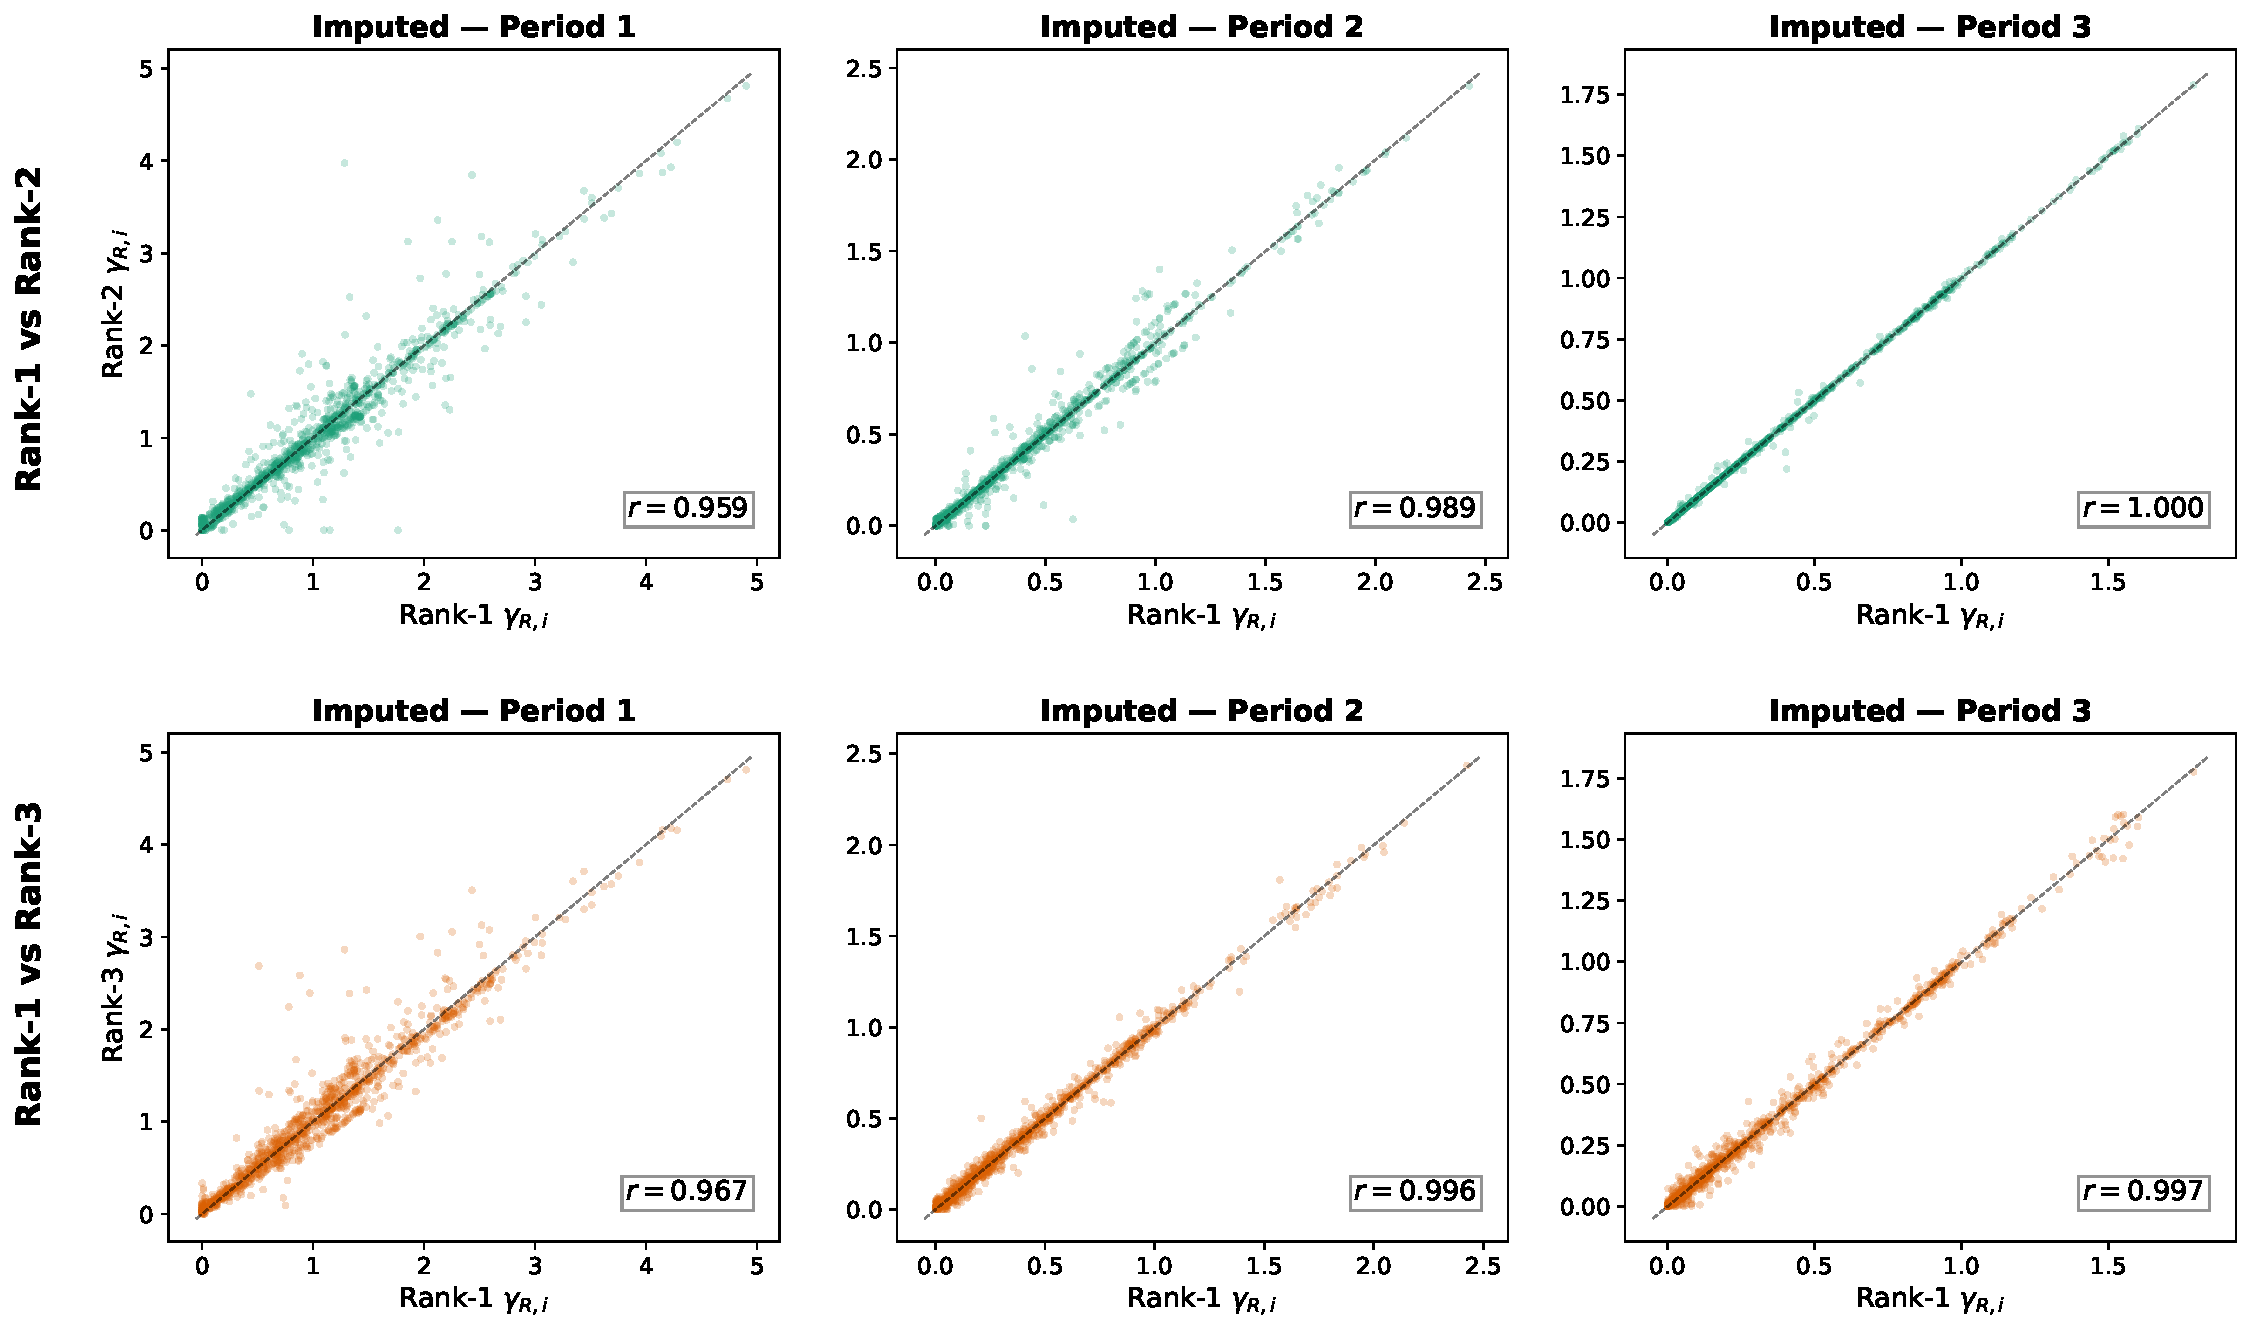
\includegraphics[width=\textwidth]{simulation_results/multiperiod_lowrank/scatter_rank1_vs_rank2_rank3_combined.png}
		\caption{Scatter plots of imputed $\gamma_{R,i}$ entries: rank-1 vs.\ rank-2 (row~1) and rank-1 vs.\ rank-3 (row~2) across three pandemic periods. High correlation confirms that higher-rank models largely agree with the rank-1 baseline on unobserved policy-region combinations.}
		\label{fig:rank1_vs_rank3_scatter}
	\end{figure}
	
	The counterfactual estimates are highly correlated across specifications. To further illustrate this stability, Figure~\ref{fig:gamma_bar_comparison} compares the rank-1, rank-2, and rank-3 estimates for the four focal regions in the paper:
	\begin{figure}[htbp]
		\centering
		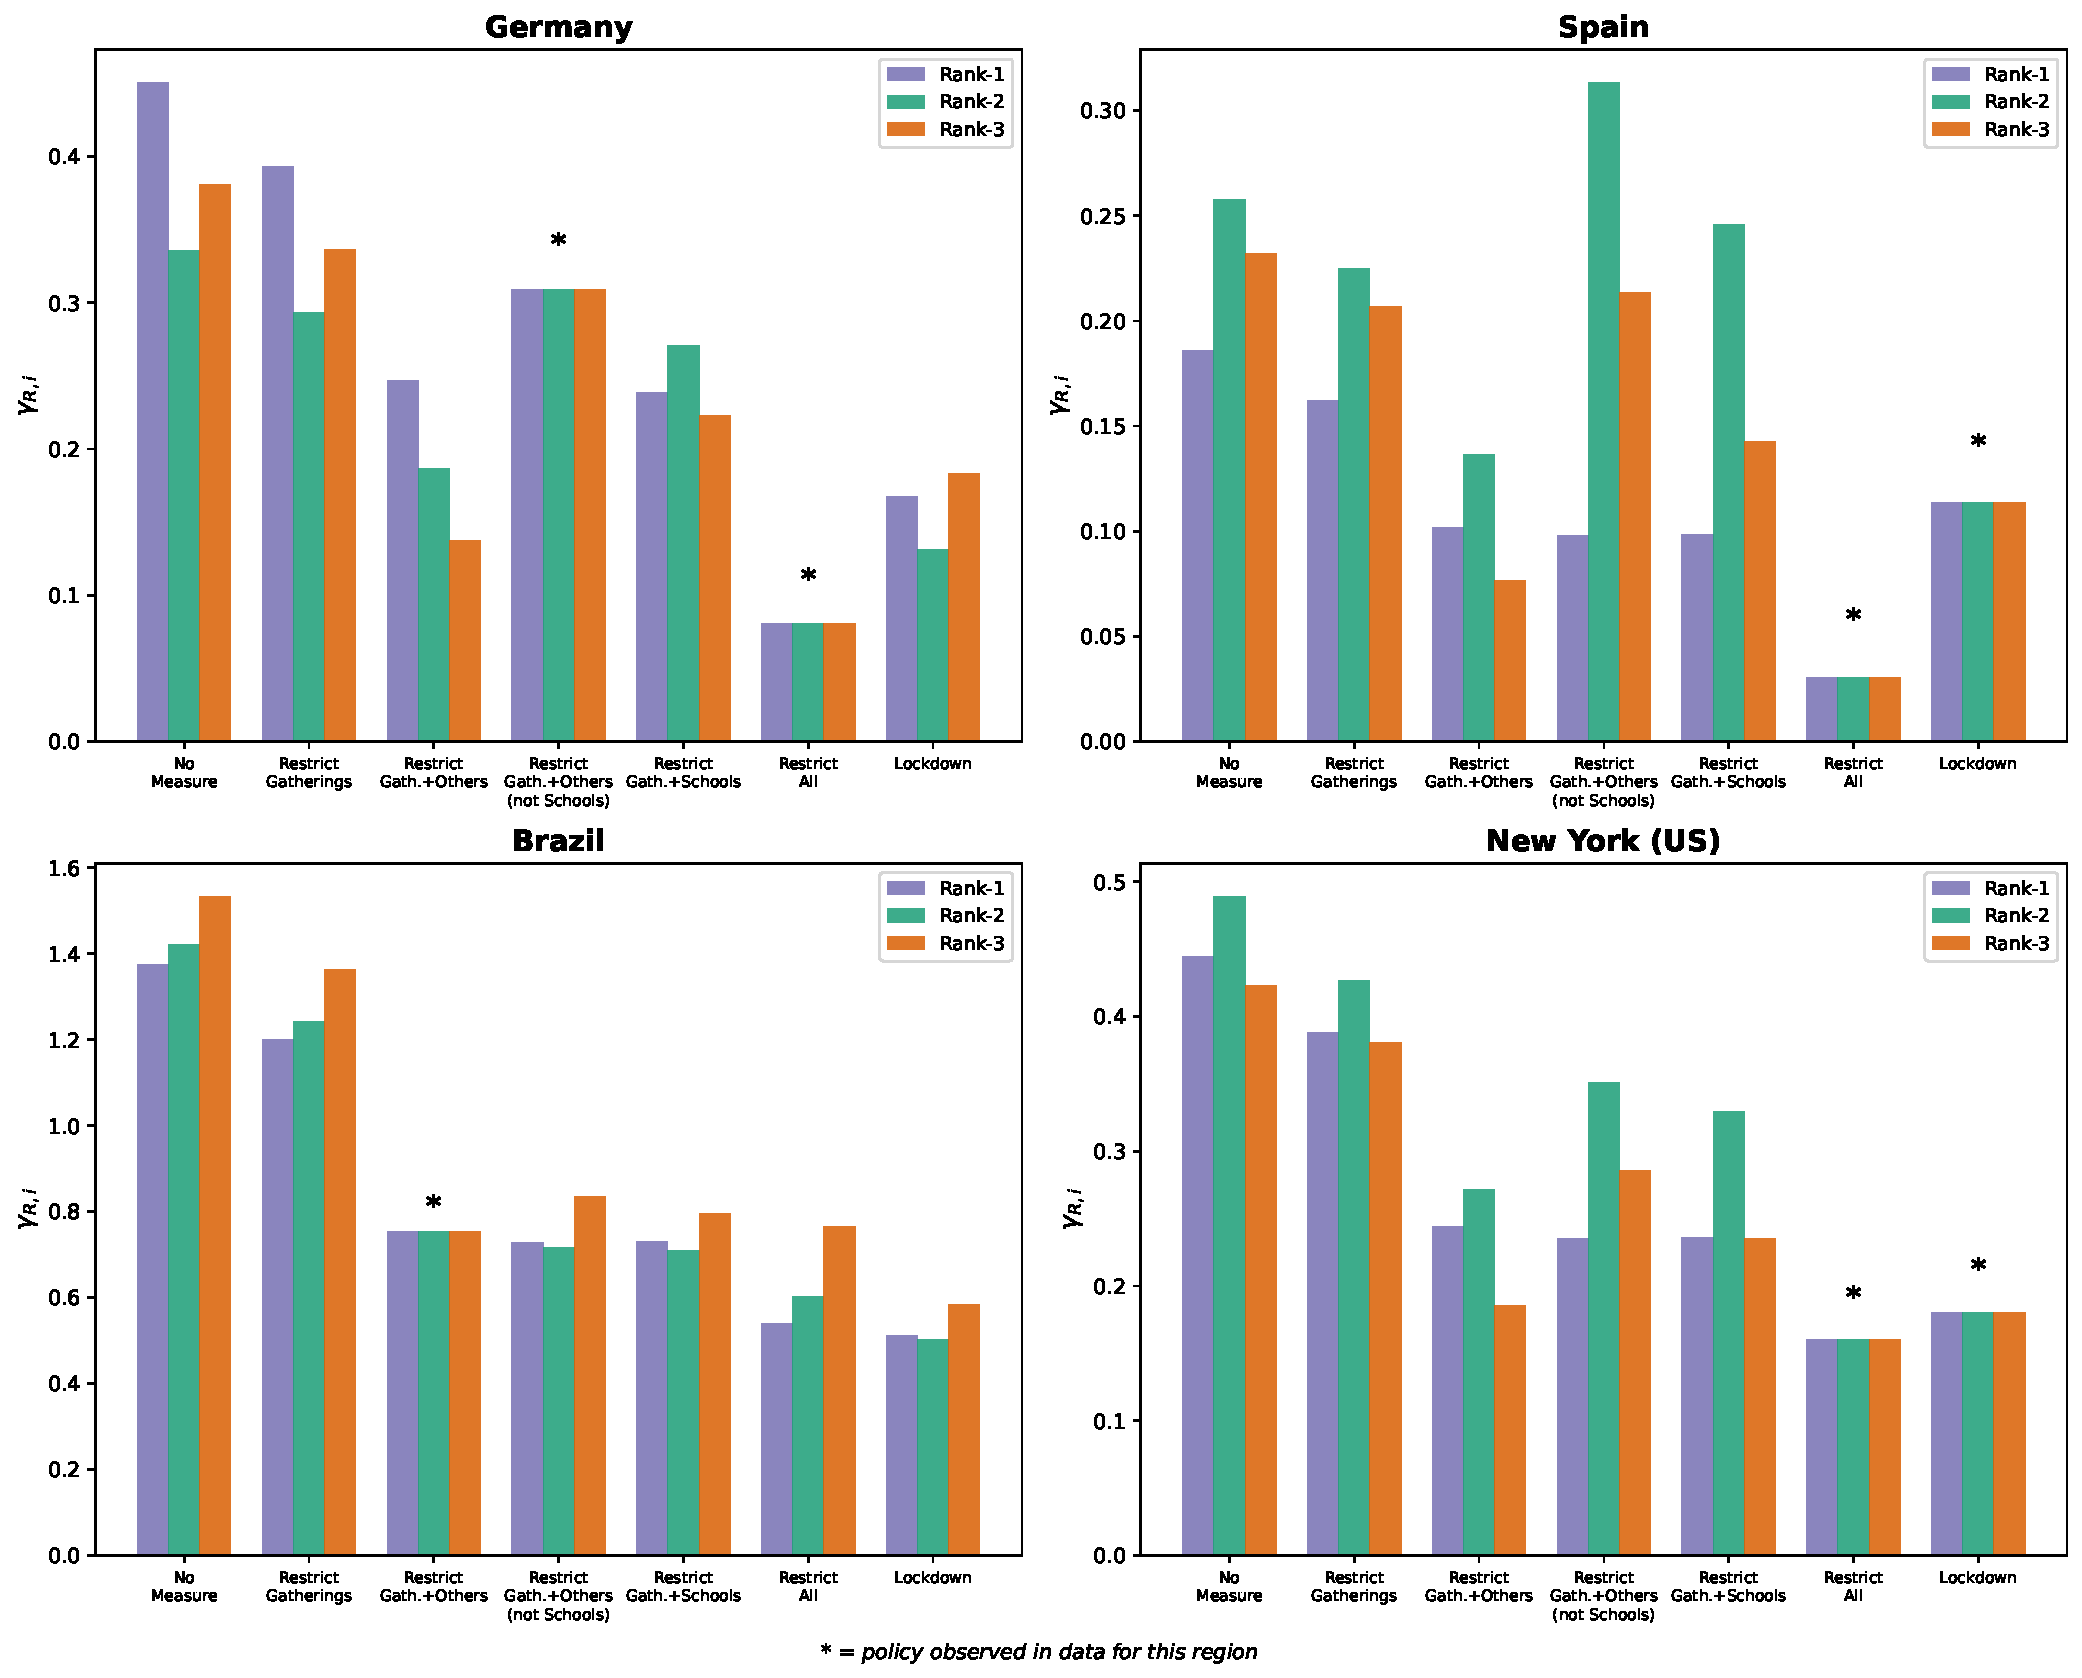
\includegraphics[width=\textwidth]{simulation_results/rank1_vs_rank3/paper_regions_gamma_comparison.png}
		\caption{Rank-1, rank-2, and rank-3 $\gamma_{R,i}$ estimates for four regions across all NPI categories (ordered by increasing severity). Policies for which observed data exists are marked with an asterisk (*).}
		\label{fig:gamma_bar_comparison}
	\end{figure}
	
	Across these 24 focal estimates, all but two differ by less than $0.05$ across the three rank specifications. Taken together, these results show that the counterfactual policy effects used in the paper are not materially altered by moving from rank~1 to rank~2 or rank~3.
	
	\textit{2. Comparison with simpler alternative specifications.}  
	The second revision shows that the rank-1 structure is not merely parsimonious, but also meaningfully improves upon simpler one-dimensional alternatives. We compare our baseline model to two natural benchmarks:
	\begin{enumerate}
		\item \textbf{Policy-only (homogeneous across regions):} $\gamma_{R,i} = \beta_i$, where $\beta_i$ is the mean of observed $\gamma_{R,i}$ values across all regions for policy $i$.
		\item \textbf{Region-only (homogeneous across policies):} $\gamma_{R,i} = \alpha_R$, where $\alpha_R$ is the mean of observed $\gamma_{R,i}$ values across all policies for region $R$.
	\end{enumerate}
	The policy-only specification ignores region-specific heterogeneity, while the region-only specification ignores policy-specific heterogeneity. Both are nested within the rank-1 model.
	
	Using the same holdout design as above, Table \ref{tab:alt_specs} reports:
	\begin{table}[H]
		\centering
		\begin{tabular}{|c|c|c|c|}
			\hline Model & 2020.03.15--2020.06.15 & 2020.06.15--2020.09.15 & 2020.09.15--2020.12.15\\\hline
			Rank-1 & $\mathbf{0.378} \pm 0.042$ & $\mathbf{0.287} \pm 0.026$ & $0.296 \pm 0.019$ \\
			Policy-only ($\beta_i$) & $0.402 \pm 0.036$ & $0.334 \pm 0.030$ & $0.291 \pm 0.023$ \\
			Region-only ($\alpha_R$) & $0.511 \pm 0.056$ & $0.387 \pm 0.050$ & $0.292 \pm 0.038$ \\\hline
		\end{tabular}
		\caption{Holdout RMSE (mean $\pm$ std.\ over 20 random splits) for three model specifications across three pandemic periods (20\% held out). Bold indicates the lowest RMSE in each period. The rank-1 model outperforms both baselines in Periods~1 and~2; all models converge in Period~3.}
		\label{tab:alt_specs}
	\end{table}
	
	These comparisons sharpen the interpretation of the rank-1 assumption. In the first two periods, the rank-1 model outperforms both benchmarks by a clear margin, indicating that both policy heterogeneity and region heterogeneity matter, and that their interaction is captured meaningfully by a single multiplicative factor. The region-only specification performs worst, which is consistent with substantial variation across NPIs. The policy-only specification performs better than the region-only specification, but still yields $6$--$16\%$ higher RMSE than the rank-1 model. In Period~3, all three models perform similarly, which is consistent with the much lower cross-region variation in policies during the later phase of the sample. Overall, these results show that the rank-1 model captures substantially more of the relevant structure than either simpler alternative, while remaining considerably more stable than higher-rank specifications.
	
	\textit{3. Connection to the low-rank counterfactual literature.}  
	The third revision is to position this assumption more clearly within the literature. Low-rank structure is widely used in counterfactual analysis for panel and observational settings with incomplete treatment support. For example, \citet{athey2021matrix} use matrix completion methods to estimate missing potential outcomes in panel data, \citet{bai2009panel} develop panel models with interactive fixed effects based on a low-rank factor structure, and \citet{moon2015linear} study linear regression models with low-rank cross-sectional dependence. Our use of a rank-1 structure is therefore not ad hoc. Rather, it is the most parsimonious member of a broader and well-established class of low-rank approximations for partially observed matrices.
	
	In summary, the revised manuscript now addresses this issue on three distinct margins. First, we show that allowing higher-rank interaction does not improve out-of-sample performance and does not materially change the counterfactual policy estimates of interest. Second, we show that the rank-1 specification substantially improves upon simpler models that ignore either policy heterogeneity or region heterogeneity. Third, we clarify that this modeling choice is consistent with a broader low-rank literature used for counterfactual analysis in related settings. For these reasons, we believe the revision now provides much stronger support for the use of the rank-1 structure as a parsimonious and empirically appropriate approximation for the policy counterfactual analysis carried out in the paper.

\item \textbf{Unaddressed potential confounding between NPIs and outcomes, as noted by the authors}
We thank the reviewer for raising this important concern. We agree that confounding is an inherent challenge in any observational study of NPI effectiveness. Because NPIs are not randomly assigned, changes in infection dynamics around policy adoption may also reflect other contemporaneous factors, including voluntary behavioral responses, seasonal variation, mobility changes, or shifts in testing intensity. In the revised manuscript, we now address this issue more directly through a new \emph{ranking stability analysis} that quantifies how much unmeasured confounding would be required to materially alter the policy rankings produced by THEMIS. The full analysis is presented in the new Appendix~\ref{app:confounding}; we summarize the main findings below.

At a high level, this analysis is designed to address the confounding concern at the level most relevant for the paper's conclusions. THEMIS is ultimately used to rank candidate policy sequences by total cost. Accordingly, the key practical question is not whether unmeasured confounding could change the absolute level of the estimated policy effects, but whether it could materially alter the \emph{relative ordering} of policies that drives the decision recommendations. The new analysis is intended to answer precisely that question.

\textit{Policy ranking stability under confounding perturbation.}  Following the logic of \citet{cinelli2020making}, we design a sensitivity analysis that directly targets the object most relevant for the paper's conclusions: the \emph{relative ordering} of candidate policies. Specifically, for each region $R$, we shrink the estimated policy-specific effects $\gamma_{R,i}$ toward their cross-policy mean
\[
\bar{\gamma}_R = \frac{1}{|\mathcal{I}|}\sum_{i\in\mathcal{I}} \gamma_{R,i}
\]
by a fraction $f \in [0,1]$, so that
\[
\gamma_{R,i}^{(f)} = (1-f)\,\gamma_{R,i} + f\,\bar{\gamma}_R.
\]
At $f=0$, we recover the original estimates. At $f=1$, all policies are assigned the same $\gamma$ within a region, so NPIs no longer have any differential effect. This perturbation therefore provides a transparent way to model the possibility that part of the observed policy contrast is driven by unmeasured confounding rather than true policy differences.

For each value of $f$, we re-simulate all $6^3 = 216$ hypothetical policy sequences through the full THEMIS pipeline and record the resulting cost ranking. We then compare the perturbed ranking to the baseline ranking at $f=0$ using two measures: the Spearman rank correlation coefficient $\rho$, and the top-$K$ overlap, defined as the fraction of the $K$ lowest-cost policies under the baseline ranking that remain in the top-$K$ set after perturbation. This construction focuses on the \emph{contrast} between policies, which is the quantity that drives the cost comparison in THEMIS, rather than the absolute level of $\gamma$, which is more directly affected by the overall transmission environment in a region.

Table \ref{tab:ranking_stability} reports the results for the four focal regions in the paper:
\begin{table}[H]
	\centering
	\begin{tabular}{|l|c|c|cc|}
		\hline
		& & $f=0.50$ & \multicolumn{2}{c|}{First $f$ at which} \\
		Region & Optimal policy & $\rho$ & optimal changes & $\rho < 0.80$ \\\hline
		Germany & Moderate early & $0.84$ & $0.20$ & $0.90$ \\
		Brazil  & Lockdown--taper & $0.99$ & $0.80$ & $0.80$ \\
		Spain   & Full lockdown   & $1.00$ & $1.00$ & $1.00$ \\
		New York & Moderate--taper & $1.00$ & $0.70$ & $1.00$ \\\hline
	\end{tabular}
	\caption{Ranking stability under confounding perturbation. $f$ is the fraction of the differential NPI effect shrunk toward the cross-policy mean, and $\rho$ is the Spearman rank correlation between the perturbed and baseline cost rankings across all 216 policies. ``First $f$ at which optimal changes'' reports the smallest $f$ for which the cost-minimizing policy differs from baseline. ``$\rho < 0.80$'' reports the smallest $f$ at which $\rho$ drops below $0.80$.}
	\label{tab:ranking_stability}
\end{table}

The results show substantial stability in three of the four focal regions. For Brazil, Spain, and New York, the ranking remains highly robust even under large perturbations. In all three regions, the Spearman correlation remains above $0.8$ through $f=0.8$, and the cost-minimizing policy is unchanged through at least $f=0.7$. Spain is especially stable: the optimal policy, full lockdown, does not change until $f=1.00$, and the rank correlation remains above $0.99$ through $f=0.90$. Thus, for these regions, even a large attenuation of the estimated differential NPI effects does not materially alter the policy conclusions delivered by THEMIS.

Germany is more sensitive, but in a way that is itself informative. In this region, the optimal policy changes at $f=0.20$, from ``Restrict Mass Gatherings and Schools--No Measure--No Measure'' to ``Authorize Schools but Restrict Mass Gatherings and Others--No Measure--No Measure.'' These two sequences are substantively close, both corresponding to moderate and time-limited interventions. This sensitivity reflects a structural feature of the German case: the baseline societal response is already strong, which yields $\gamma$ values below $0.18$ for \emph{all} NPI categories and leaves relatively little room for further differentiation across interventions. Even so, the broader ranking structure remains stable. The rank correlation remains above $0.75$ throughout the full perturbation sweep, and the qualitative conclusion that moderate, time-limited interventions dominate both prolonged lockdown and no action remains unchanged through $f=0.40$.

Overall, this sensitivity analysis shows that the paper's main policy conclusions are not being driven by particularly sensitive estimates of the differential NPI effects. In three of the four focal regions, one can eliminate one half or more of the estimated policy contrast without materially changing the ranking. Even in the most sensitive region, the recommended policy changes only within a narrow set of closely related moderate interventions, while the broader substantive conclusion remains intact.

We agree, of course, that no sensitivity analysis can fully eliminate the possibility of unmeasured confounding in an observational setting. At the same time, we believe this new analysis substantially strengthens the manuscript by showing that the policy rankings produced by THEMIS are stable to large attenuations in the estimated differential NPI effects. For this reason, while the revised manuscript does not eliminate the usual identification concerns of an observational study, it does show that the paper's substantive policy conclusions are robust to substantial weakening of the estimated differential NPI effects.

\item \textbf{The additive treatment of different NPI effects (highlighted by Reviewer 1)}

Thank you for raising this point. We agree that, in a setting with multiple overlapping non-pharmaceutical interventions, it is important to clarify exactly what object the model treats as a ``policy effect.'' In the revised manuscript, we now make this explicit. The THEMIS framework does \emph{not} assume that the effects of individual NPIs enter additively. Rather, each policy $i \in \mathcal{I}$ is defined as a mutually exclusive and collectively exhaustive intervention bundle, and the corresponding quantity $\gamma_{R,i}$ captures the joint effect of that entire bundle in region $R$.

Specifically, the model is not written at the level of separate school-closure, gathering-restriction, and travel-restriction coefficients that are then summed. Instead, each day in each region is mapped to exactly one policy category, and the estimated infection-rate reduction factor for that category reflects the combined effect of all interventions active within that bundle. Thus, for example, the estimated effect for ``Restrict Mass Gatherings and Schools'' is the effect of that bundle as implemented in practice, not the sum of a standalone school-closure effect and a standalone mass-gathering effect. We apologize that this was not made clearer in the previous version.

To make this construction transparent, we now describe more carefully how the policy categories are built from the Oxford COVID-19 Government Response Tracker (OxCGRT) \cite{hale2021global}. The OxCGRT records multiple dimensions of government response, including school closures (C1), workplace closures (C2), cancellation of public events (C3), restrictions on gatherings (C4), closure of public transport (C5), stay-at-home requirements (C6), restrictions on internal movement (C7), and international travel controls (C8), each with a severity level and geographic scope flag. We binarize these indicators using the thresholds listed in Table~\ref{tab:oxford_mapping}, and then aggregate them into two composite features:
\[
\text{Restrict Mass Gatherings} = \mathbf{1}[\text{C3} \lor \text{C4} \lor \text{C5}],
\qquad
\text{Others} = \mathbf{1}[\text{C2} \lor \text{C7} \lor \text{C8}].
\]
Using four building blocks---Schools (C1), Mass Gatherings, Others, and Stay-at-Home (C6)---we assign each region-day to exactly one of seven policy categories.

\begin{table}[htbp!]
	\centering
	\small
	\begin{tabular}{|l|c|c|c|c|l|}
		\hline
		\textbf{THEMIS Policy Category} & \textbf{Schools} & \textbf{Mass Gath.} & \textbf{Others} & \textbf{C6} & \textbf{Rule} \\\hline
		(1) No Measure & 0 & 0 & 0 & 0 & sum $= 0$ \\
		(2) Restrict Mass Gatherings & 0 & 1 & 0 & 0 & sum $= 1$, MG on \\
		(3) Others Only & 0 & 0 & $\geq 1$ & 0 & MG off, C6 off \\
		(4) Mass Gath.\ + Schools & 1 & 1 & 0 & 0 & sum $= 2$, C1+MG \\
		(5) Mass Gath.\ + Others (no Schools) & 0 & 1 & $\geq 1$ & 0 & C1 off, MG on, C6 off \\
		(6) Mass Gath.\ + Schools + Others & 1 & 1 & $\geq 1$ & 0 & sum $> 2$, C1+MG on, C6 off \\
		(7) Stay-at-Home / Lockdown & --- & --- & --- & 1 & C6 on \\\hline
	\end{tabular}
	\caption{Mapping from OxCGRT binary indicators to the 7 MECE policy categories used in THEMIS. ``Mass Gath.'' denotes the composite $\mathbf{1}[\text{C3} \lor \text{C4} \lor \text{C5}]$; ``Others'' denotes $\mathbf{1}[\text{C2} \lor \text{C7} \lor \text{C8}]$. Stay-at-home (C6 $= 1$) takes precedence and maps to Lockdown regardless of other indicators.}
	\label{tab:oxford_mapping}
\end{table}

This mapping was developed in coordination with the Oxford team and is intended to reflect the intervention bundles that were most commonly co-implemented during the early pandemic. The resulting categories are mutually exclusive and collectively exhaustive by construction. For this reason, the estimated $\gamma_{R,i}$ values should be interpreted as bundle-level effects rather than as additive combinations of underlying NPI coefficients.

At the same time, we agree that the choice of policy partition is important. Even if the model does not impose additivity across individual NPIs, one may still ask whether the conclusions depend materially on the coarseness of the seven-category grouping. To address this concern directly, we now add a new sensitivity analysis based on a more granular policy partition.

\textit{Sensitivity to a more granular partition.}  
In the appendix of the revised manuscript, we construct a finer mutually exclusive and collectively exhaustive partition that splits the two broadest original categories---Restrict Mass Gatherings, Schools and Others, and Lockdown---according to within-category stringency intensity. These two categories contain the majority of region-days in the data and cover the widest range of policy severity, making them the natural candidates for further subdivision. Specifically, we compute the sum of the raw OxCGRT severity levels (C1--C8, prior to flag-based binarization) and split observations at the global median stringency into ``Moderate'' and ``Strict'' sub-categories. The remaining five categories each represent a more homogeneous set of measures and are retained without splitting. This yields a 9-category partition, each element of which is a strict refinement of one of the original seven categories.

\begin{table}[h!]
	\centering
	\small
	\begin{tabular}{|c|l|l|c|c|}
		\hline
		\textbf{ID} & \textbf{Granular Category} & \textbf{Original Category} & \textbf{Cutoff} & \textbf{Regions Obs.} \\\hline
		G1 & No Measure & (1) No Measure & --- & 0 \\
		G2 & Restrict Mass Gatherings & (2) Restrict Mass Gath. & --- & 0 \\
		G3 & MG + Schools & (4) MG + Schools & --- & 5 \\
		G4 & Others Only & (3) Others Only & --- & 42 \\
		G5 & MG + Others & (5) MG + Others (no Schools) & --- & 38 \\
		G6 & MG + Schools + Others -- Moderate & (6) MG + Schools + Others & $\leq 16$ & 70 \\
		G7 & MG + Schools + Others -- Strict & (6) MG + Schools + Others & $> 16$ & 107 \\
		G8 & Lockdown -- Moderate & (7) Lockdown & $\leq 20$ & 108 \\
		G9 & Lockdown -- Strict & (7) Lockdown & $> 20$ & 48 \\\hline
	\end{tabular}
	\caption{The 9 granular MECE policy categories, their mapping to the original 7 categories, the stringency cutoff used for the Moderate/Strict split (global median of $\sum_{k=1}^{8} \text{C}k_{\text{raw}}$), and the number of regions (out of 210) in which each was observed for at least 10 days during March 15--June 15, 2020.}
	\label{tab:granular_policies}
\end{table}

This refinement is intended to capture within-category heterogeneity that is suppressed by the original coarser grouping. For example, the original ``Restrict Mass Gatherings, Schools and Others'' category encompasses observations ranging from moderate combinations of closures to near-lockdown bundles. The granular partition allows these cases to be distinguished while preserving the same bundle-based logic as the original specification.

We then re-estimate the $\gamma_{R,i}$ matrix under the 9-category partition across all 210 regions and repeat the same holdout-RMSE exercise used in our earlier low-rank analysis. Table~\ref{tab:granular_rmse} reports the results.

\begin{table}[htbp!]
	\centering
	\begin{tabular}{|c|cc|}
		\hline
		& \multicolumn{2}{c|}{Holdout RMSE} \\
		Rank $l$ & Original (7 cat.) & Granular (9 cat.) \\\hline
		1 & $0.378$ & $0.400$ \\
		2 & $0.420$ & $0.439$ \\
		3 & $0.391$ & $0.410$ \\\hline
	\end{tabular}
	\caption{Holdout RMSE (20\% held out, averaged over 20 splits) for rank-$l$ models under the original 7-category and the granular 9-category policy partitions. The rank-1 model achieves the lowest holdout RMSE in both cases.}
	\label{tab:granular_rmse}
\end{table}

The same qualitative pattern continues to hold. Under both the original and the granular policy partitions, the rank-1 model provides the best out-of-sample fit. Thus, allowing a more refined policy classification does not change the effectiveness of the rank-1 estimation procedure used in THEMIS.

We also evaluate whether the finer partition materially changes the epidemiological predictions used in the paper. Using the granular $\gamma_{R,i}$ estimates, we re-run the DELPHI model for the four focal regions under their \emph{actual} policy sequences during March 15--June 15, 2020, mapping each day to its granular category. Where a region has observed $\gamma$ for a granular sub-category, we use the observed value directly. For unobserved sub-categories whose parent category is observed, we retain the parent-category estimate; ALS-imputed values are used only when neither level has observations. Table~\ref{tab:granular_predictions} compares the resulting cumulative predictions.

\begin{table}[H]
	\centering
	\begin{tabular}{|l|rr|c|rr|c|}
		\hline
		& \multicolumn{3}{c|}{Cumulative Cases} & \multicolumn{3}{c|}{Cumulative Deaths} \\
		Region & Original & Granular & $\Delta$\% & Original & Granular & $\Delta$\% \\\hline
		Germany & 144{,}063 & 152{,}288 & 5.7\% & 6{,}044 & 6{,}386 & 5.7\% \\
		Spain & 118{,}075 & 117{,}999 & 0.1\% & 13{,}784 & 13{,}778 & 0.0\% \\
		Brazil & 582{,}815 & 582{,}815 & 0.0\% & 26{,}949 & 26{,}949 & 0.0\% \\
		New York & 130{,}855 & 116{,}747 & 10.8\% & 11{,}501 & 10{,}392 & 9.6\% \\\hline
	\end{tabular}
	\caption{Predicted cumulative cases and deaths (March 15--June 15, 2020) under the original 7-category versus granular 9-category policy partition. $\Delta$\% is the absolute percentage difference.}
	\label{tab:granular_predictions}
\end{table}

The predicted trajectories remain close across the two specifications. Spain and Brazil exhibit essentially no difference ($\leq 0.1\%$), because these regions' active policies during the simulation period fall entirely within unsplit categories or have directly observed granular $\gamma$ values that coincide with the original estimates. Germany and New York show modest deviations of $5.7\%$ and $10.8\%$ respectively, driven by the within-category stringency split of the ``Restrict All'' category, which assigns slightly different $\gamma$ values to the Moderate and Strict sub-periods. In all four regions, the direction and magnitude of predicted cumulative cases and deaths are closely aligned.

Figure~\ref{fig:granular_predictions} reports the full cumulative case trajectories under the original and granular partitions.

\begin{figure}[H]
	\centering
	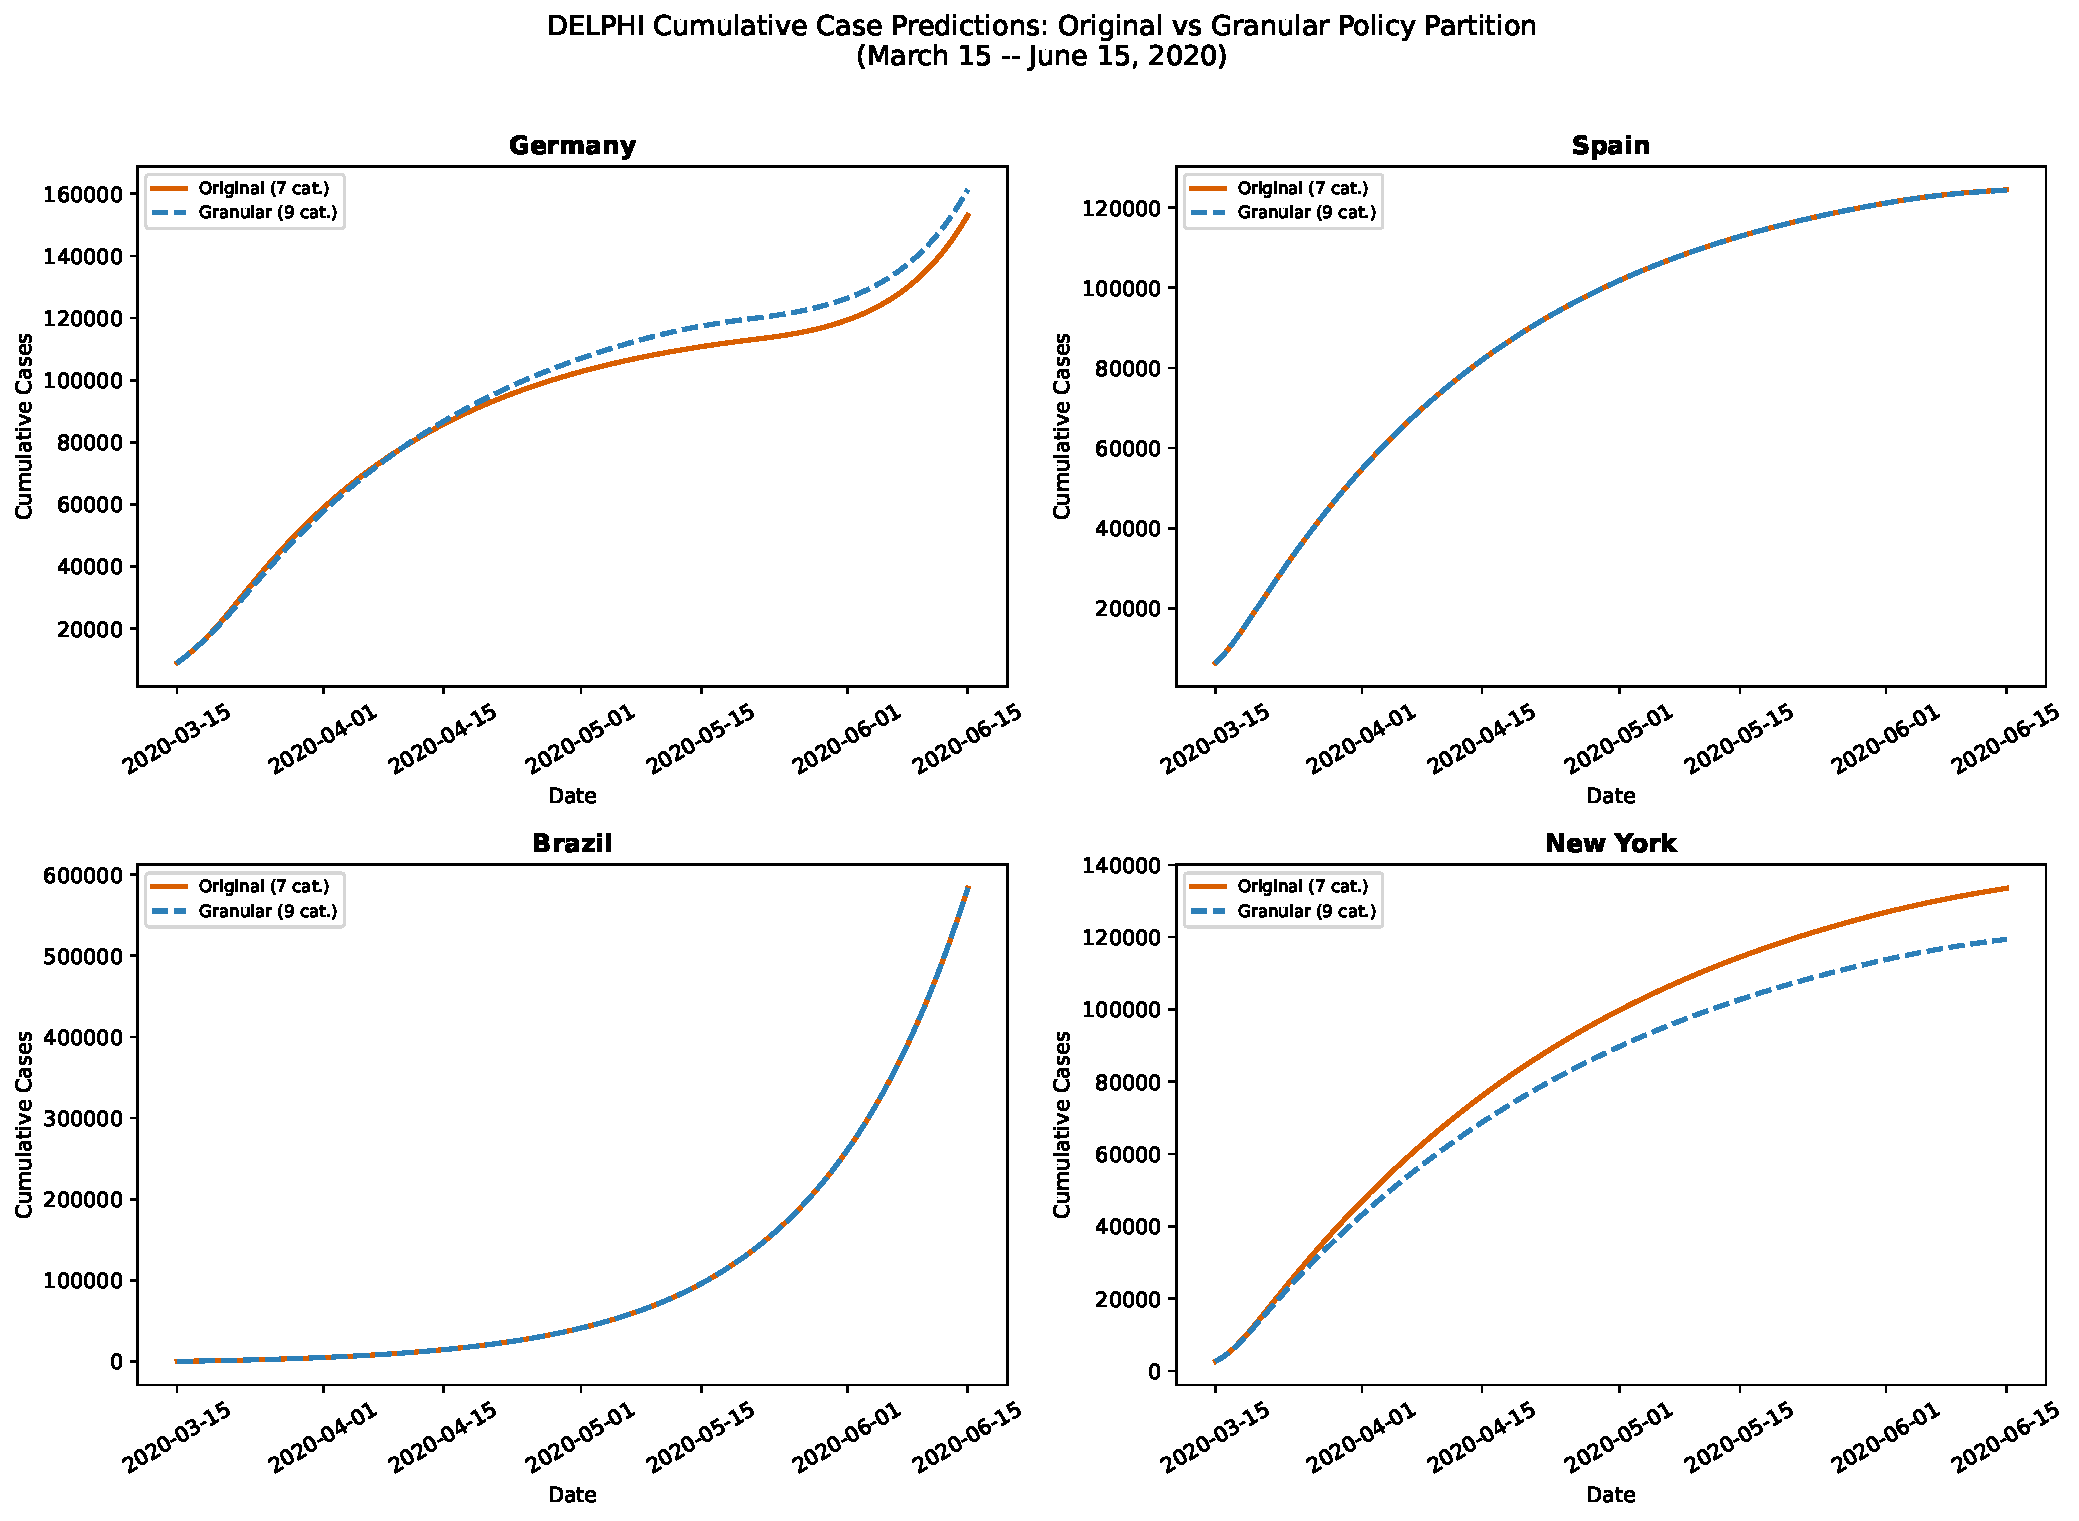
\includegraphics[width=\textwidth]{simulation_results/granular_policies/combined_prediction_comparison.png}
	\caption{DELPHI cumulative case predictions under the original 7-category (solid) and granular 9-category (dashed) policy partitions for the March 15--June 15, 2020 period. The curves track closely in all four regions.}
	\label{fig:granular_predictions}
\end{figure}

Taken together, these revisions address the concern on two levels. First, we clarify that the THEMIS model does not assume additive effects of individual NPIs. The basic object of analysis is a bundle-level policy category, and $\gamma_{R,i}$ is the joint effect of that category as implemented in practice. Second, we show that refining the policy partition to allow more within-category heterogeneity does not materially change either the estimation results or the substantive conclusions of the paper. The revised manuscript therefore clarifies both the interpretation of the policy effects and the robustness of the framework to a more granular treatment of intervention bundles.

    \item \textbf{The assumption that policies maintain consistent effects across different seasons (policy-season interaction)}
    
    We agree that demonstrating the temporal stability of the estimated policy effects is essential. If the $\gamma_{R,i}$ values estimated in one period do not produce accurate predictions when applied to a different period, the counterfactual analysis would be unreliable. We therefore follow the AE's suggestion and conduct an out-of-sample time-transfer test: we train the DELPHI model and estimate all $\gamma_{R,i}$ on one period, then evaluate prediction accuracy in a \emph{subsequent, non-overlapping} period using only the policy-driven counterfactual curve for $\gamma$.
    
    \textbf{Experimental design.} We train DELPHI on March 15--June 15, 2020 (Period~1) and evaluate predictions on June 15--September 15, 2020 (Period~2). For the evaluation period, we construct the THEMIS counterfactual $\gamma$ curve using the \emph{actual} policies implemented in each region during Period~2, combined with the $\gamma_{R,i}$ estimates from Period~1. Specifically, we define $\gamma_R^P(t)$ as a piecewise constant function of the region-specific reduction factors:
    \begin{equation}
    	\gamma_R^P(t)=\begin{cases}
    		\gamma_{R,i_0} & t_0\leq t<t_1\\
    		\gamma_{R,i_1} & t_1\leq t<t_2\\ 
    		\vdots & \vdots \\
    		\gamma_{R,i_{k-1}} & t_{k-1}\leq t<t_k\\ 
    	\end{cases}
    \end{equation}
    where $i_j$ is the NPI in effect in Region $R$ during time window $[t_j, t_{j+1})$ in Period~2. If the policy effects are temporally stable, this piecewise curve---constructed entirely from Period~1 estimates---should yield accurate case predictions in Period~2.
    
    We compare THEMIS against four benchmarks: (i) \textbf{DELPHI}, the base epidemiological model re-fit on the training period data with its flexible, nonparametric $\gamma(t)$ curve; (ii) \textbf{DELPHI-constant}, which freezes $\gamma$ at its training-period endpoint value throughout evaluation (i.e., no policy adjustment); (iii) \textbf{DELPHI-lookahead}, a non-causal oracle that re-fits DELPHI on both training and evaluation periods jointly, serving as an upper bound on achievable accuracy; and (iv) \textbf{SIR} and \textbf{SEIRD}, standard compartmental models (susceptible--infected--recovered, and susceptible--exposed--infected--recovered--deceased, respectively) without any policy-adjustment mechanism. The SIR and SEIRD baselines are included to demonstrate that simple compartmental models cannot match THEMIS's accuracy. All DELPHI-family models share the same underlying dynamics; the only difference is how $\gamma(t)$ is specified during the evaluation period. We report the mean absolute percentage error (APE) of daily cumulative case predictions over the evaluation window. We use simulated annealing for global optimization to ensure robust parameter estimates across all models.
    
	\textbf{Period~1 $\to$ Period~2 results.} Table~\ref{tab:time_transfer_main} reports the results for the four regions analyzed in the paper (Germany, Spain, Brazil, and New York), trained on Period~1 (March--June 2020) and evaluated on Period~2 (June--September 2020).
    
    \begin{table}[H]
    	\centering
    	\begin{tabular}{|l|cccccc|}
    		\hline
    		& \multicolumn{6}{c|}{Mean daily APE, cases (\%)} \\
    		Region & DELPHI-LA & DELPHI & THEMIS & DELPHI-const. & SIR & SEIRD \\\hline
    		Brazil     & $49.3$ & $66.3$ & $\mathbf{74.4}$ & $75.2$ & $4248.1$ & $2504.3$ \\
    		Germany    & $9.2$  & $14.0$ & $\mathbf{34.7}$ & $34.7$ & $5843.3$ & $1171.2$ \\
    		Spain      & $29.9$ & $22.7$ & $\mathbf{44.3}$ & $53.7$ & $2304.0$ & $290.6$ \\
    		New York   & $3.6$  & $8.2$  & $\mathbf{28.1}$ & $28.8$ & $6.5$    & $571.8$ \\\hline
    		\textbf{Mean}   & $23.0$ & $27.8$ & $\mathbf{45.4}$ & $48.1$ & $3100.5$ & $1134.5$ \\
    		\textbf{Median} & $19.6$ & $18.3$ & $\mathbf{39.5}$ & $44.2$ & $3276.0$ & $871.5$ \\\hline
    	\end{tabular}
    	\caption{Out-of-sample time-transfer test: models trained on Period~1 (Mar--Jun 2020), evaluated on Period~2 (Jun--Sep 2020). THEMIS uses the piecewise $\gamma_R^P(t)$ constructed from Period~1 policy estimates. Bold indicates THEMIS outperforms DELPHI-constant.}
    	\label{tab:time_transfer_main}
    \end{table}
    
    In all four regions, THEMIS outperforms DELPHI-constant: in Spain, THEMIS reduces the case APE from $53.7\%$ to $44.3\%$ ($-9.4$~pp), and in Brazil from $75.2\%$ to $74.4\%$. On average, THEMIS reduces the case APE from $48.1\%$ to $45.4\%$ relative to DELPHI-constant, a $2.7$ percentage point improvement; at the median, the improvement is $4.7$~pp ($44.2\% \to 39.5\%$). The SIR and SEIRD models---which lack any policy-adjustment mechanism---produce errors that are one to two orders of magnitude larger (mean APEs of $3{,}101\%$ and $1{,}135\%$ respectively), confirming that simple compartmental models cannot capture the policy-driven dynamics that THEMIS exploits.
    
    \textbf{Expanded validation on 40 regions.} To ensure that our results are not driven by the specific choice of regions, we extend the Period~1$\to$Period~2 analysis to a broader set of 40 regions spanning five continents. These regions include major European countries (Spain, Germany, Italy, France, Sweden, Turkey, Switzerland, Ireland, Austria, Denmark, Finland, Norway, Czechia), North American provinces and states (Canada--Ontario, Canada--Quebec, 10 U.S.\ states), Asia-Pacific countries (Malaysia, Thailand, New Zealand, Australia), the Caribbean (Cuba, Dominican Republic), and small nations (Andorra, San Marino, Iceland, Liechtenstein). We use simulated annealing for all DELPHI parameter fits.
    
    \begin{table}[H]
    	\centering
    	\begin{tabular}{|l|cccccc|}
    		\hline
    		& \multicolumn{6}{c|}{Mean daily APE, cases (\%)} \\
    		Statistic & DELPHI-LA & DELPHI & THEMIS & DELPHI-const. & SIR & SEIRD \\\hline
    		Mean APE   & $12.0$ & $15.6$ & $\mathbf{36.4}$ & $41.3$ & $1315.3$ & $889.1$ \\
    		Median APE & $8.2$  & $13.6$ & $\mathbf{31.5}$ & $36.2$ & $178.5$  & $192.0$ \\
    		THEMIS wins & --- & --- & \multicolumn{2}{c|}{$39/40$ ($97.5\%$)} & --- & --- \\\hline
    	\end{tabular}
    	\caption{Out-of-sample time-transfer test on 40 regions. THEMIS outperforms DELPHI-constant on 39 of 40 regions, reducing mean APE by $4.9$~pp and median APE by $4.7$~pp.}
    	\label{tab:time_transfer_expanded}
    \end{table}
    
    Across all 40 regions, THEMIS outperforms DELPHI-constant on 39 of 40 regions ($97.5\%$), reducing the mean case APE from $41.3\%$ to $36.4\%$ ($-4.9$~pp) and the median from $36.2\%$ to $31.5\%$ ($-4.7$~pp). The improvements are particularly pronounced in regions that experienced significant policy changes between Period~1 and Period~2: for example, the Dominican Republic, U.S.--North Dakota, and U.S.--South Dakota each show double-digit percentage-point reductions. In regions where policies remained relatively stable across periods, THEMIS and DELPHI-constant produce nearly identical predictions---as expected, since the policy-driven $\gamma_R^P(t)$ converges to the constant $\gamma$ when policy does not change. The SIR and SEIRD baselines produce errors that are one to two orders of magnitude larger, confirming that simple compartmental models without policy-adjustment mechanisms cannot capture the dynamics of a subsequent pandemic period.
    
    Notably, for several regions THEMIS's piecewise counterfactual curve approaches or matches the accuracy of DELPHI's nonparametric $\gamma(t)$, despite the fact that THEMIS uses only policy-level information (which NPI was in effect on each day) rather than fitting the curve freely to the data. This provides strong evidence that the $\gamma_{R,i}$ estimates from Period~1 capture genuine policy-driven variation in infection rates that \emph{transfers across time}.
    
    These results are detailed in the new Appendix~\ref{app:time_transfer}. We view this analysis as direct empirical evidence that the estimated policy effects are temporally stable: NPI effectiveness estimated in the first pandemic wave retains predictive power three months later, supporting the validity of THEMIS's counterfactual simulations across seasons.

\end{enumerate}

\rcomment{
In addition, I strongly agree with both reviewers that the current managerial insights remain anticipated and too high-level to be truly actionable. A more in-depth exploration that uncovers more nuanced insights could substantially strengthen the paper's contribution. Reviewer 1 in particular offered numerous valuable suggestions regarding stylized assumptions and potential improvement directions that the authors should address in revision.
}

Thank you for this important feedback. We fully agree that the original manuscript stopped at descriptive simulation and did not extract the concrete, reusable guidance that would make THEMIS truly useful to operational planners. In this revision, we have substantially expanded the paper's prescriptive contribution by embedding THEMIS into an actionable decision-making pipeline. We present three complementary modules below.

\textbf{(A) Decision-rule extraction via interpretable classification.} We use the full $6^3=216$ simulation output from THEMIS to train interpretable decision trees (CART) that distill the cost-optimal policy structure into human-readable if--then rules. We label each simulated 3-month sequence as \emph{near-optimal} if its total cost (economic + humanitarian) falls in the lowest 15\% of all sequences in that region, and \emph{dominated} otherwise. To identify rules that \emph{generalize across regions} rather than per-country prescriptions, we begin with a pooled tree trained on all $4 \times 216 = 864$ region--sequence rows, then report per-region trees as supporting detail.

\emph{Pooled cross-regional tree with region--policy interaction features.} The key methodological choice is that each row's features describe \emph{the policy as it acts in that region}, not the region in isolation. For each (region, sequence) pair we construct 16 features: severity-based summaries of the sequence ($s_1, s_2, s_3$, average $\bar s$, severity trend $s_3 - s_1$, indicators for starting strict and de-escalating), and \emph{region--policy interaction} attributes that quantify the sequence's footprint in that region. The interaction features are: the GDP impact in percentage of monthly GDP of the month-$t$ NPI in that region ($g_1, g_2, g_3$) and the cumulative 3-month GDP impact $G = g_1 + g_2 + g_3$, the maximum month-level GDP impact, the month-1 employment impact $e_1$ and cumulative employment impact $E = e_1 + e_2 + e_3$, and---most importantly---the \emph{intensity ratio} $\rho_t = g_t / g_{\text{Lock}}$ that expresses the month-$t$ NPI's GDP impact as a fraction of Lockdown's GDP impact in that same region. The intensity ratio is a country-agnostic policy attribute: $\rho = 0$ for No Measure, $\rho = 1$ for Lockdown, and the same NPI category yields very similar $\rho$ across regions (e.g.\ Restrict Mass Gatherings + Schools yields $\rho \in [0.679, 0.691]$ for all four regions; Sch+MG+Oth yields $\rho \in [0.270, 0.286]$). A rule expressed in $\rho$ therefore transfers directly to any new region for which lockdown's GDP impact can be estimated.

The pooled tree (depth~3, minimum leaf size~10, 5-fold CV accuracy~$=0.795$) is reported in Figure~\ref{fig:pooled_tree}. Three near-optimal leaves emerge, all defined by region--policy interaction features rather than region indicators:
\begin{table}[H]
	\centering
	\small
	\begin{tabular}{|p{0.5cm}|p{10.0cm}|c|c|c|}
		\hline
		\textbf{\#} & \textbf{Cross-country rule (pooled tree)} & \textbf{Purity} & \textbf{$n$} & \textbf{Regions} \\\hline
		1 & IF $\rho_1 \in (0.271, 0.687]$ AND $E \leq 1.05\%$ & 90\% & 10 & DE \\
		2 & IF $\rho_1 > 0.687$ AND $G \leq 47.15\%$ AND $E \leq 1.35\%$ & 100\% & 15 & DE, BR, US-NY \\
		3 & IF $\rho_1 > 0.687$ AND $G > 47.15\%$ & 100\% & 17 & ES \\\hline
	\end{tabular}
	\caption{Near-optimal leaves of the pooled cross-regional CART tree, reported as country-agnostic rules in policy-attribute space. $\rho_1 = g_1 / g_{\text{Lock}}$ is the intensity ratio of the month-1 NPI; $G = g_1 + g_2 + g_3$ is the cumulative 3-month GDP impact (\%); $E$ is the cumulative employment impact (\%). The first column is the rule; the last column lists which of the four regions contribute samples to that leaf. Feature importances at the root: $\rho_1 = 0.51$, $E = 0.25$, $G = 0.24$ (no region indicator features in the model; the tree is region-blind).}
	\label{tab:pooled_rules}
\end{table}

\begin{figure}[H]
	\centering
	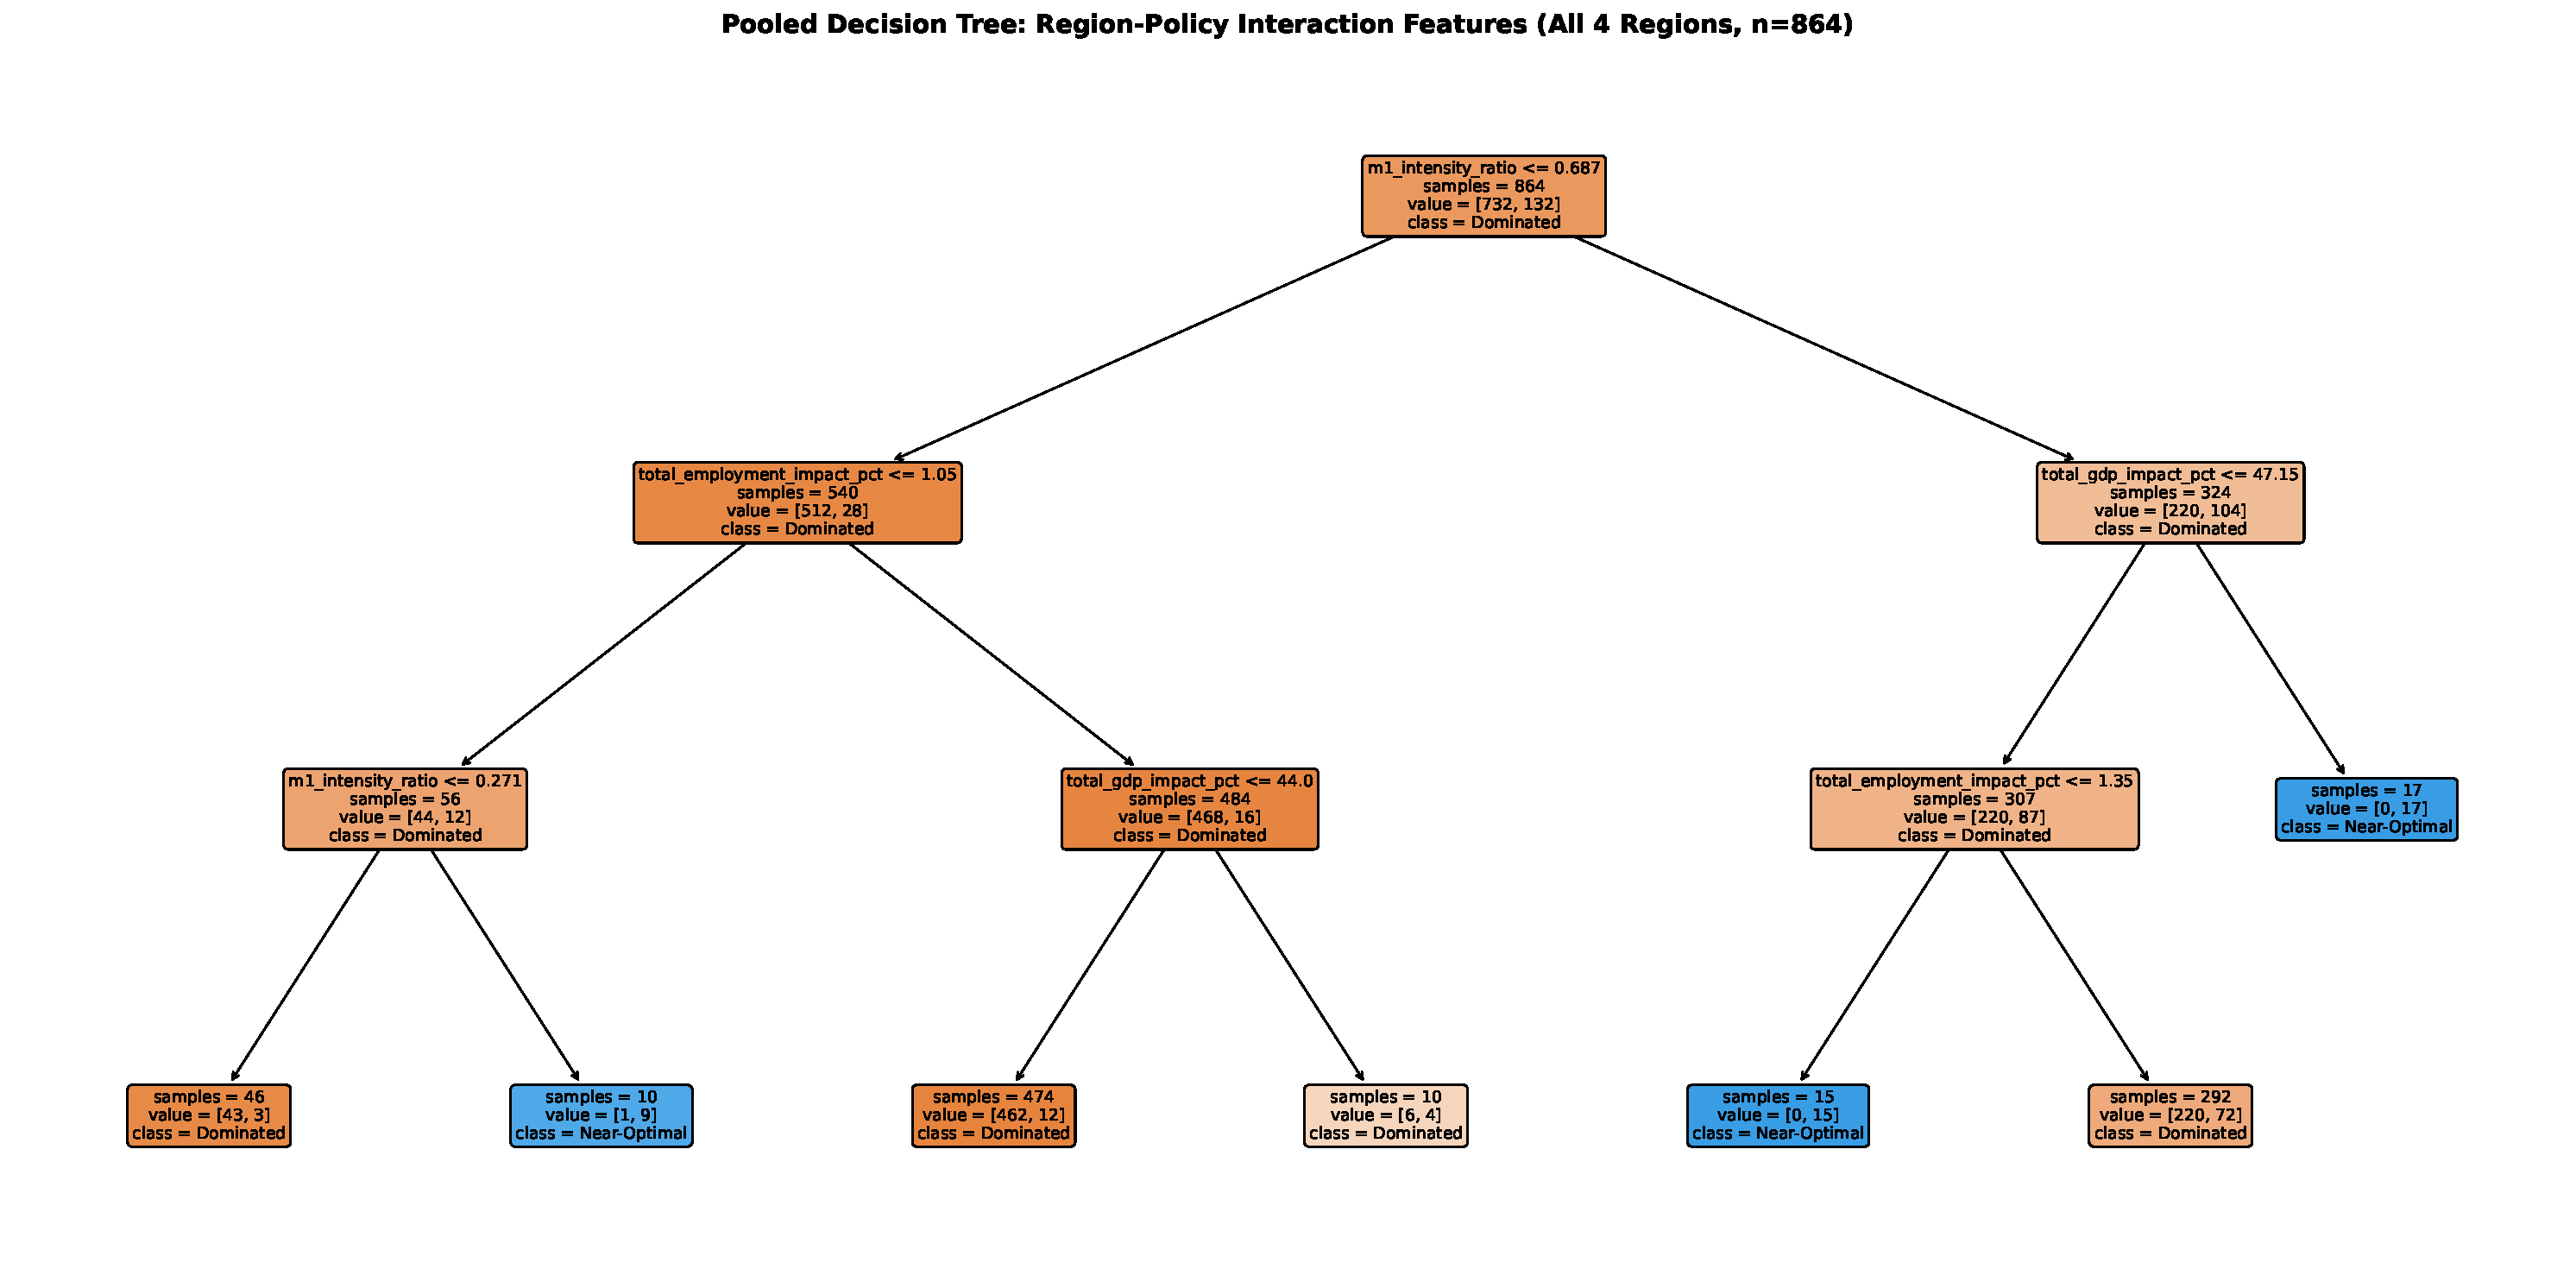
\includegraphics[width=\textwidth]{simulation_results/decision_rules/decision_tree_pooled.png}
	\caption{Pooled cross-regional CART tree trained on $4 \times 216 = 864$ simulation rows with 16 region--policy interaction features. The root split is on $\rho_1$ (the month-1 NPI's GDP impact relative to Lockdown), at the boundary $\rho_1 = 0.687$. Both subtrees lead to additional splits on cumulative GDP impact $G$ and cumulative employment impact $E$. The three near-optimal leaves (blue) correspond to: (Leaf~1) moderate-intensity month~1 with low aggregate labor disruption; (Leaf~2) strict-then-relax sequences with bounded cumulative GDP impact; and (Leaf~3) sustained strict sequences in regions where the disease threat justifies the cumulative cost.}
	\label{fig:pooled_tree}
\end{figure}

These three rules together yield a single, country-portable structural insight: \emph{a near-optimal sequence either keeps the month-1 NPI's intensity ratio in $(0.271, 0.687]$ with aggregate labor disruption below $1.05\%$, or it pushes month-1 strictness above $\rho_1 = 0.687$.} The first regime selects the Restrict Mass Gatherings + Schools NPI in DE (the only region where the 10--30\% intensity range yields any near-optimal sequences). The second regime then partitions on the cumulative GDP impact $G$: when $G \leq 47\%$, the sequence must relax in months~2--3 (the strict-then-relax archetype, near-optimal in DE, BR, US-NY); when $G > 47\%$, sustained strictness is near-optimal (only in ES, where humanitarian costs dominate by a factor of $\sim 32\times$). Critically, none of these rules names a region: any decision-maker who can estimate $\rho_1$, $G$, and $E$ for their setting can apply the rules directly.

\emph{Cross-country escalation rule.} The pooled tree implies a sharp generalizable trajectory rule. Pooling all near-optimal sequences by month-1 intensity bin (Table~\ref{tab:cross_country_escalation}, Figure~\ref{fig:cross_country_escalation}), the de-escalation pattern is universal across all four regions: at every intensity bin where any region admits a near-optimal sequence, the dominant trajectory is $s_3 < s_1$. No region admits a near-optimal sequence with month-1 intensity below $10\%$ of Lockdown's GDP impact, and the 30--55\% bin (corresponding to schools-open NPIs) is also empty across all four regions---a finding directly implying that closing schools is structurally necessary for any near-optimal sequence in our four very different regions.

\begin{table}[H]
	\centering
	\small
	\begin{tabular}{|l|c|c|c|c|c|c|}
		\hline
		\textbf{Month-1 intensity bin} & \textbf{$n$ near-optimal} & \textbf{\# regions} & \textbf{Avg $s_1$} & \textbf{Avg $s_2$} & \textbf{Avg $s_3$} & \textbf{\% de-escalate} \\\hline
		$\rho_1 < 10\%$ & 0 & 0/4 & --- & --- & --- & --- \\
		$10\% \leq \rho_1 < 30\%$ & 14 & 1/4 & 2.57 & 1.86 & 0.93 & 92.9\% \\
		$30\% \leq \rho_1 < 55\%$ & 0 & 0/4 & --- & --- & --- & --- \\
		$55\% \leq \rho_1 < 80\%$ & 73 & 4/4 & 3.40 & 3.11 & 2.19 & 87.7\% \\
		$80\% \leq \rho_1 \leq 100\%$ & 45 & 4/4 & 5.00 & 2.82 & 2.07 & 97.8\% \\\hline
	\end{tabular}
	\caption{Cross-country escalation rule: trajectory of near-optimal sequences as a function of the month-1 NPI intensity ratio $\rho_1 = g_1 / g_{\text{Lock}}$. ``Avg $s_t$'' is the average severity in month $t$ (0 = None, 5 = Lockdown) across all near-optimal sequences in the bin; ``\% de-escalate'' is the fraction of those sequences with $s_2 < s_1$ or $s_3 < s_2$. Two intensity bins ($<10\%$ and $30$--$55\%$) contain \emph{no} near-optimal sequences in any of the four regions, indicating that those NPI severities (No Measure and Sch+MG+Oth respectively) are structurally dominated for the COVID-class threat.}
	\label{tab:cross_country_escalation}
\end{table}

\begin{figure}[H]
	\centering
	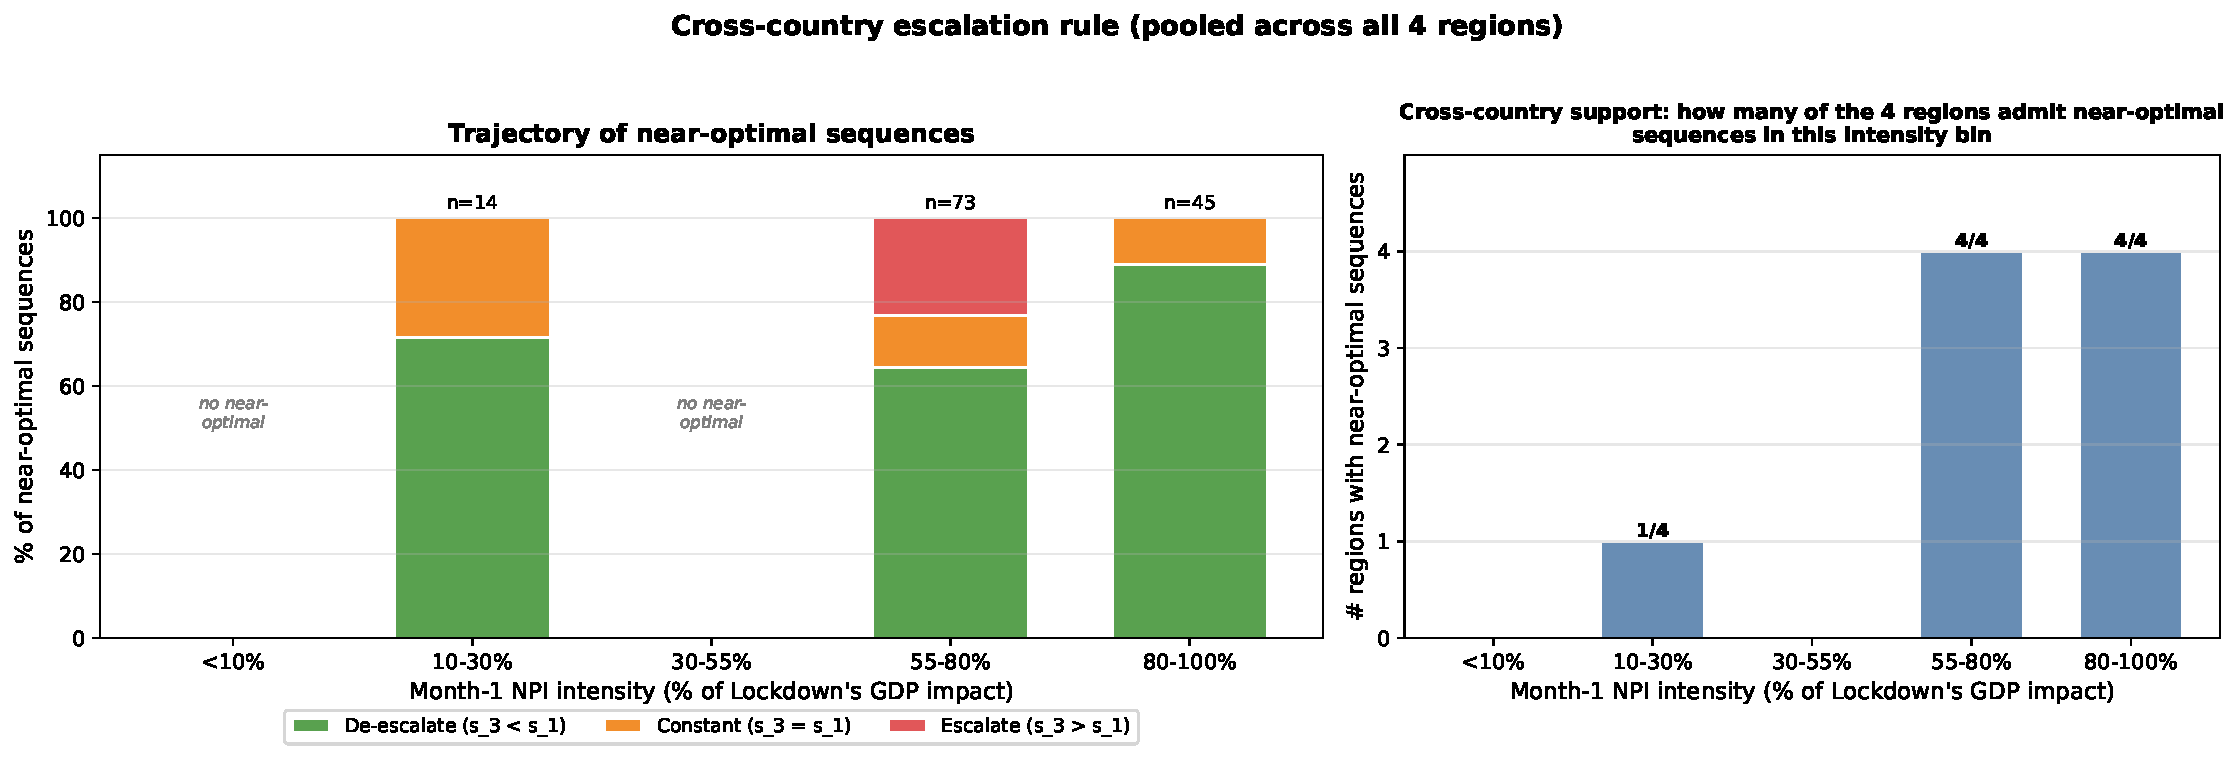
\includegraphics[width=\textwidth]{simulation_results/decision_rules/cross_country_escalation.png}
	\caption{Cross-country escalation rule. \textbf{Left:} stacked bar of escalation patterns among near-optimal sequences, broken down by month-1 NPI intensity bin and pooled across all four regions. ``De-escalate'' = $s_3 < s_1$, ``Constant'' = $s_3 = s_1$, ``Escalate'' = $s_3 > s_1$. \textbf{Right:} how many of the four regions admit at least one near-optimal sequence in each intensity bin. Two bins are completely empty (No Measure-class and the Sch+MG+Oth bracket), and only the strict ($\rho_1 \in [55\%, 80\%]$) and Lockdown-class ($\rho_1 \geq 80\%$) bins are supported in every region.}
	\label{fig:cross_country_escalation}
\end{figure}

The combined message of the pooled tree and escalation analysis is operationally crisp: a structurally near-optimal 3-month NPI sequence has month-1 intensity ratio $\rho_1 \geq 0.55$ (i.e.\ at least as restrictive as Restrict Mass Gatherings + Schools) and de-escalates over time, except in regions where the humanitarian/economic cost ratio is large enough (cf.\ Insight~3 in \S below) to justify sustained strict NPIs.

\emph{Per-region trees as supporting detail.} For completeness we also report per-region trees in Figure~\ref{fig:decision_trees} and Table~\ref{tab:decision_rules}; their CV accuracy is somewhat higher (DE~87\%, BR~77\%, ES~79\%, US-NY~85\%) than the pooled tree, but their leaves describe region-specific severity thresholds and are not directly transferable.

\begin{figure}[H]
	\centering
	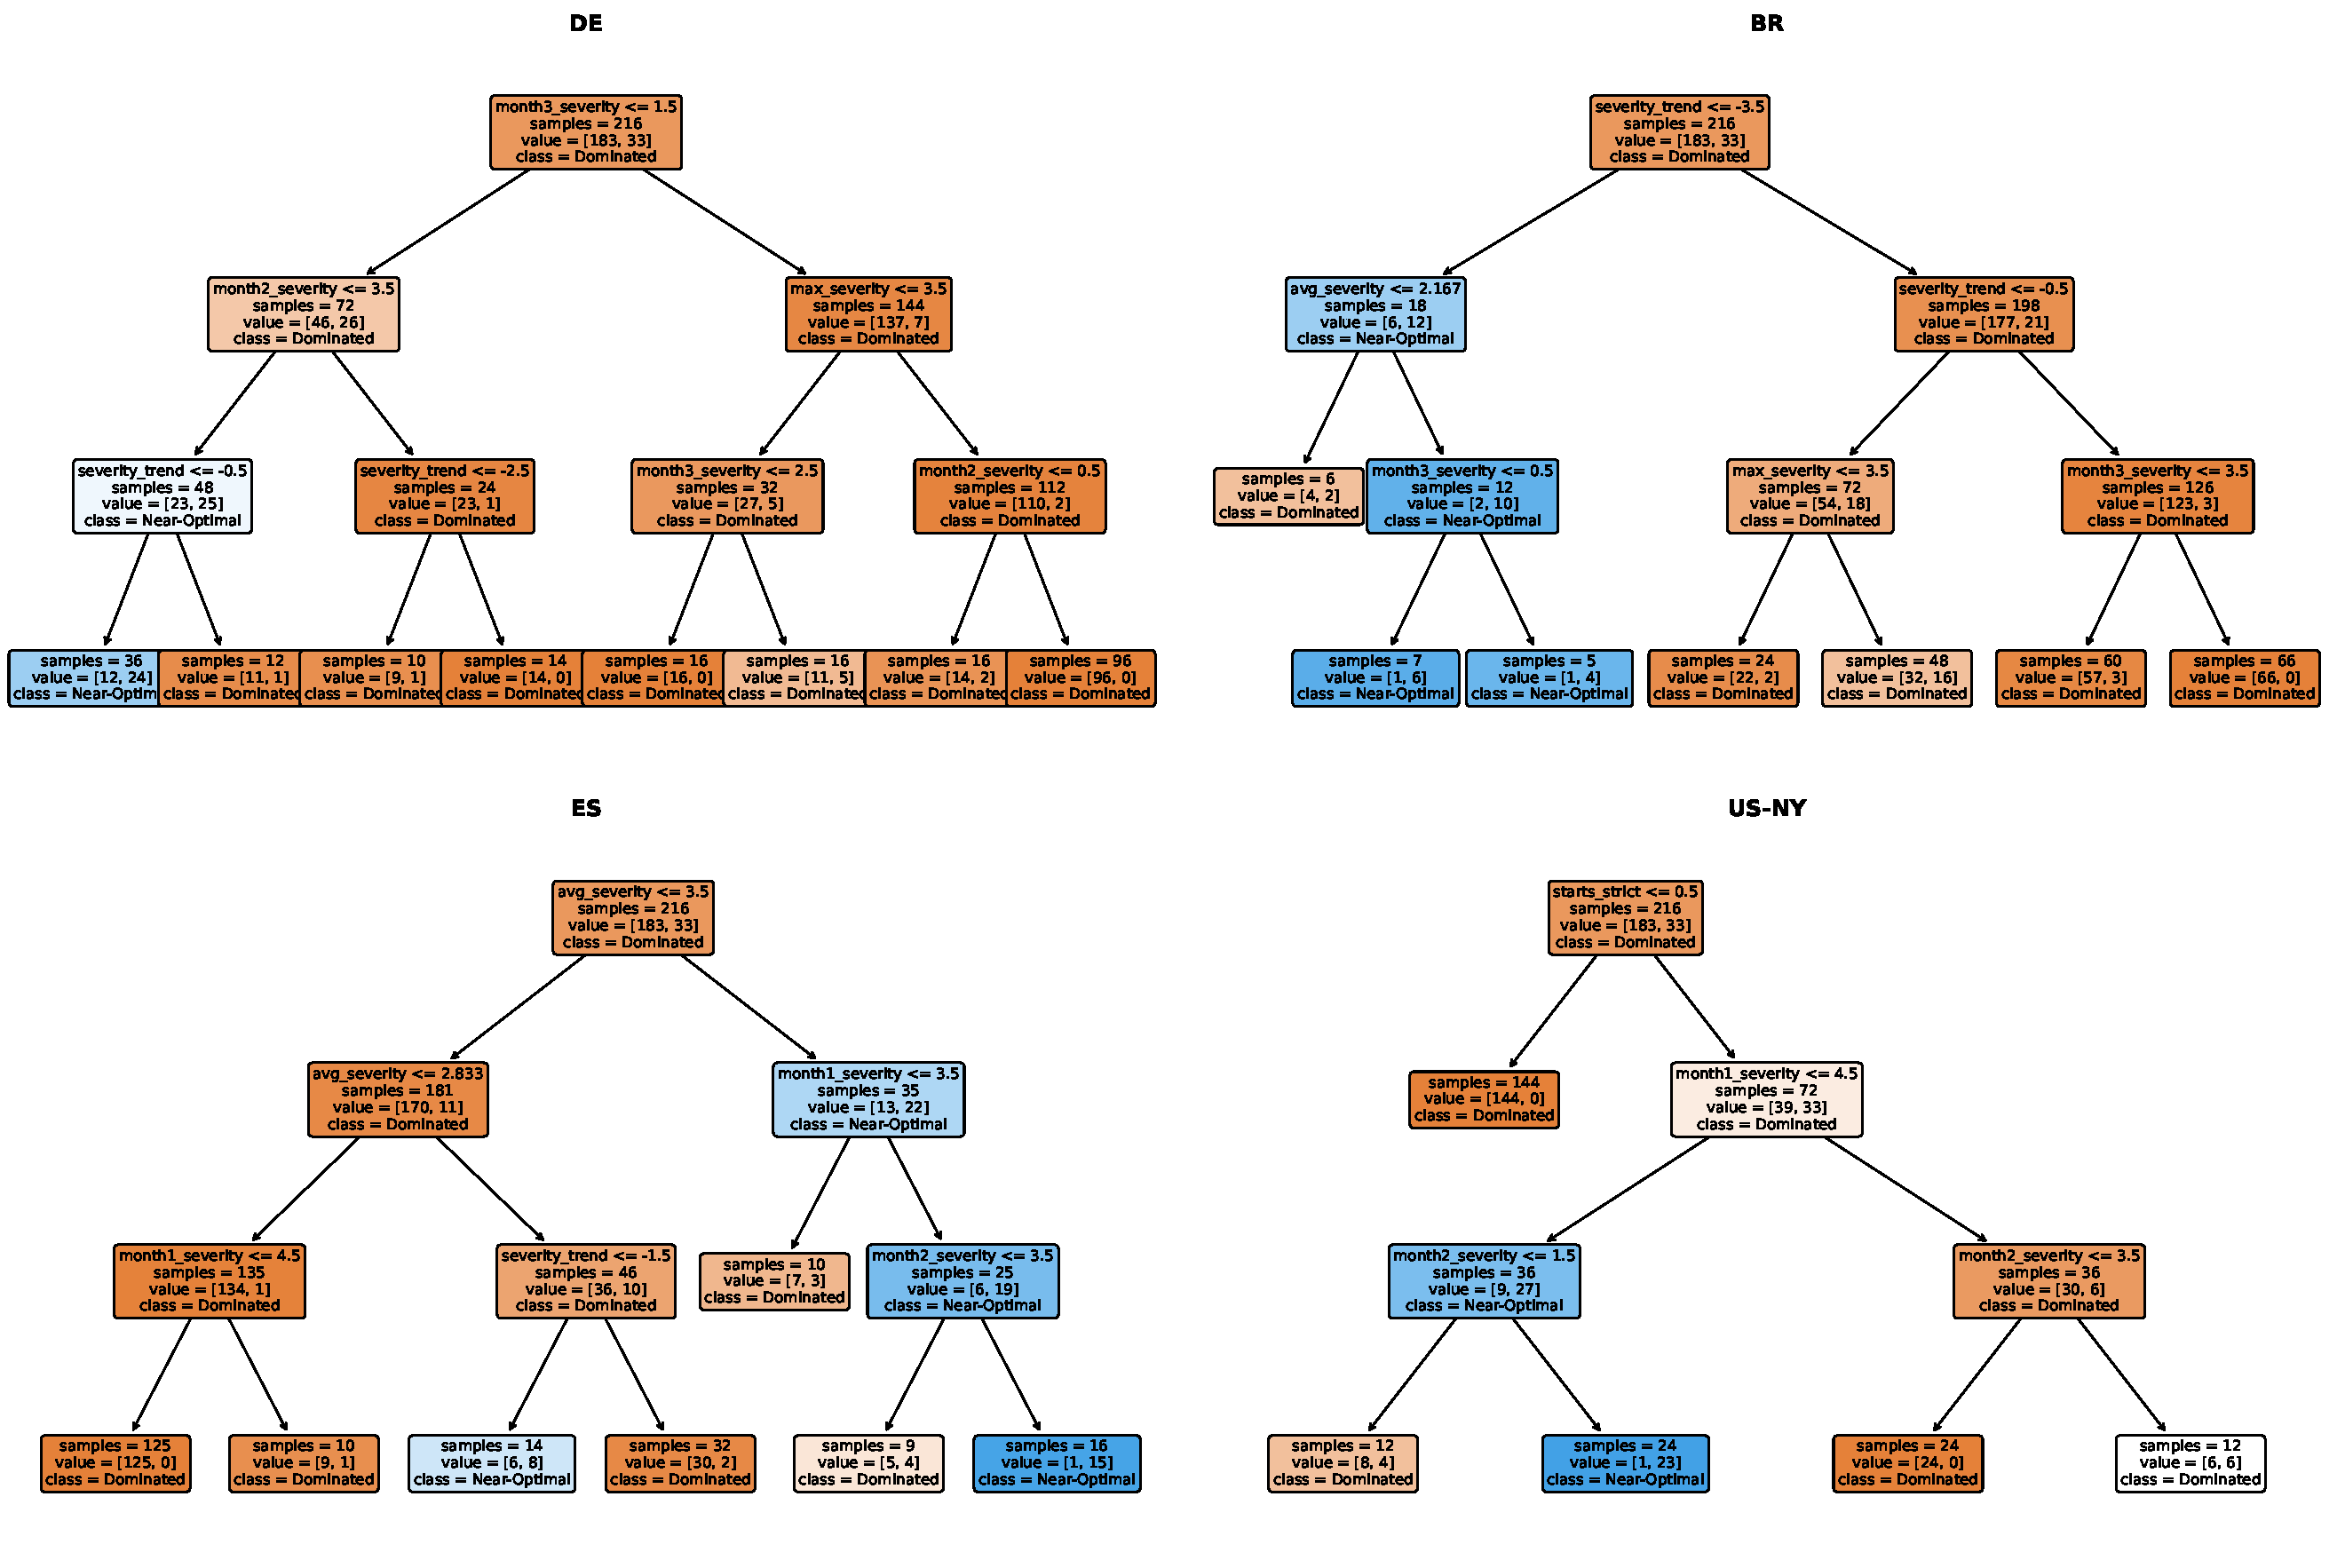
\includegraphics[width=\textwidth]{simulation_results/decision_rules/decision_trees_combined.png}
	\caption{Per-region CART trees (depth $\leq 3$, supporting detail) classifying 216 sequences each as near-optimal (top 15\% by total cost, green) vs.\ dominated (orange). These trees achieve marginally higher per-region CV accuracy than the pooled tree, but their splits are in raw severity space and do not transfer across regions. The pooled tree of Figure~\ref{fig:pooled_tree} sacrifices a modest amount of per-region accuracy for portable, country-agnostic rules.}
	\label{fig:decision_trees}
\end{figure}

\begin{table}[H]
	\centering
	\small
	\begin{tabular}{|l|p{7.5cm}|c|c|}
		\hline
		\textbf{Region} & \textbf{Per-region rule (path to near-optimal leaf)} & \textbf{Purity} & \textbf{$n$} \\\hline
		Germany & IF $s_3 \leq 1.5$ AND $s_2 \leq 3.5$ AND trend $\leq -0.5$ & 67\% & 36 \\\hline
		Brazil & IF trend $\leq -3.5$ AND $\bar{s} > 2.17$ AND $s_3 \leq 0.5$ & 86\% & 7 \\
		Brazil & IF trend $\leq -3.5$ AND $\bar{s} > 2.17$ AND $s_3 > 0.5$ & 80\% & 5 \\\hline
		Spain & IF $\bar{s} \leq 3.5$ AND $\bar{s} > 2.83$ AND trend $\leq -1.5$ & 57\% & 14 \\
		Spain & IF $\bar{s} > 3.5$ AND $s_1 > 3.5$ AND $s_2 > 3.5$ & 94\% & 16 \\\hline
		New York & IF starts\_strict AND $s_1 \leq 4.5$ AND $s_2 > 1.5$ & 96\% & 24 \\\hline
	\end{tabular}
	\caption{Near-optimal leaves of the per-region CART trees of Figure~\ref{fig:decision_trees}. Notation: $s_1, s_2, s_3$ = month-by-month severity, $\bar s$ = average severity, trend $= s_3 - s_1$. These per-region rules are reported for completeness and consistency with the pooled tree of Figure~\ref{fig:pooled_tree}; the pooled tree gives the country-portable rules (Table~\ref{tab:pooled_rules}).}
	\label{tab:decision_rules}
\end{table}

\emph{Novel quantitative insights from the simulation data.} Beyond the tree-based classification, the $4 \times 216$ simulation grid reveals several non-obvious structural findings:

\begin{enumerate}
\item \textbf{Lockdown dominates No\_Measure in total cost for \emph{every} region.} Despite its economic burden, Lockdown produces lower total cost than No\_Measure across all four regions. However, the implied cost per life saved varies by over 60$\times$: \$1.33M/life in Germany vs.\ \$0.02M/life in Spain. This quantifies the intuition that the case for lockdown is stronger in high-mortality settings---but the finding that lockdown is cheaper even in Germany (where economic costs are highest) is non-trivial and depends on THEMIS's integration of death, hospitalization, and mental-health valuations.

\item \textbf{Month-2 sensitivity is non-monotone in month-1 strictness.} Conventional wisdom suggests that a strict month-1 ``locks in'' a trajectory, making subsequent decisions less consequential. Our data show the opposite for some regions: after a month-1 Lockdown, the coefficient of variation (CV) of total costs across month-2/3 choices is \emph{highest} for Spain (CV = 0.94) and \emph{lowest} for Brazil (CV = 0.09). In Spain, even after Lockdown, the choice between de-escalating to No\_Measure vs.\ sustaining Lockdown in month~2 changes total cost by \$92T---because the pandemic trajectory is so steep that any relaxation leads to massive mortality rebound. In Brazil, the trajectory is contained enough after month-1 Lockdown that month-2 choices barely matter (range = \$37B). This has a direct operational implication: policymakers in high-mortality regions \emph{cannot} assume that an initial lockdown buys time for relaxed decision-making.

\item \textbf{The humanitarian/economic dominance ratio determines policy structure.} At the optimal policy, the ratio of humanitarian to economic costs varies from 0.9$\times$ (Brazil, economic-dominated) to 31.7$\times$ (Spain, humanitarian-dominated), with Germany at 1.4$\times$ and New York at 5.8$\times$. Brazil is the \emph{only} region where economic costs exceed humanitarian at the optimum, explaining why it is the only region with a developing-nation-specific policy pattern (different month-1 optimal from the rest). This ratio is computable from THEMIS's cost functions before simulation and can serve as a fast diagnostic for classifying new regions' policy regimes.

\item \textbf{Marginal cost of severity reveals non-monotone returns.} Figure~\ref{fig:marginal_costs} plots the average economic, humanitarian, and total cost as a function of month-1 NPI severity. The total cost curve is U-shaped for Germany (minimum at severity 2 = MG+Sch) but monotonically decreasing for Spain (minimum at severity 5 = Lockdown). Furthermore, the step from severity 4 (MG+Sch+Oth) to severity 5 (Lockdown) adds \$6.8B in economic costs for Germany but saves only \$2.5B in humanitarian costs---a \emph{net} increase. For Spain, the same step saves \$25.5T in humanitarian costs while adding only \$2.6B in economic costs. This ``diminishing returns'' threshold, identifiable from the marginal cost curves, provides a quantitative criterion for when the most restrictive NPI is no longer cost-justified.
\end{enumerate}

\begin{figure}[H]
	\centering
	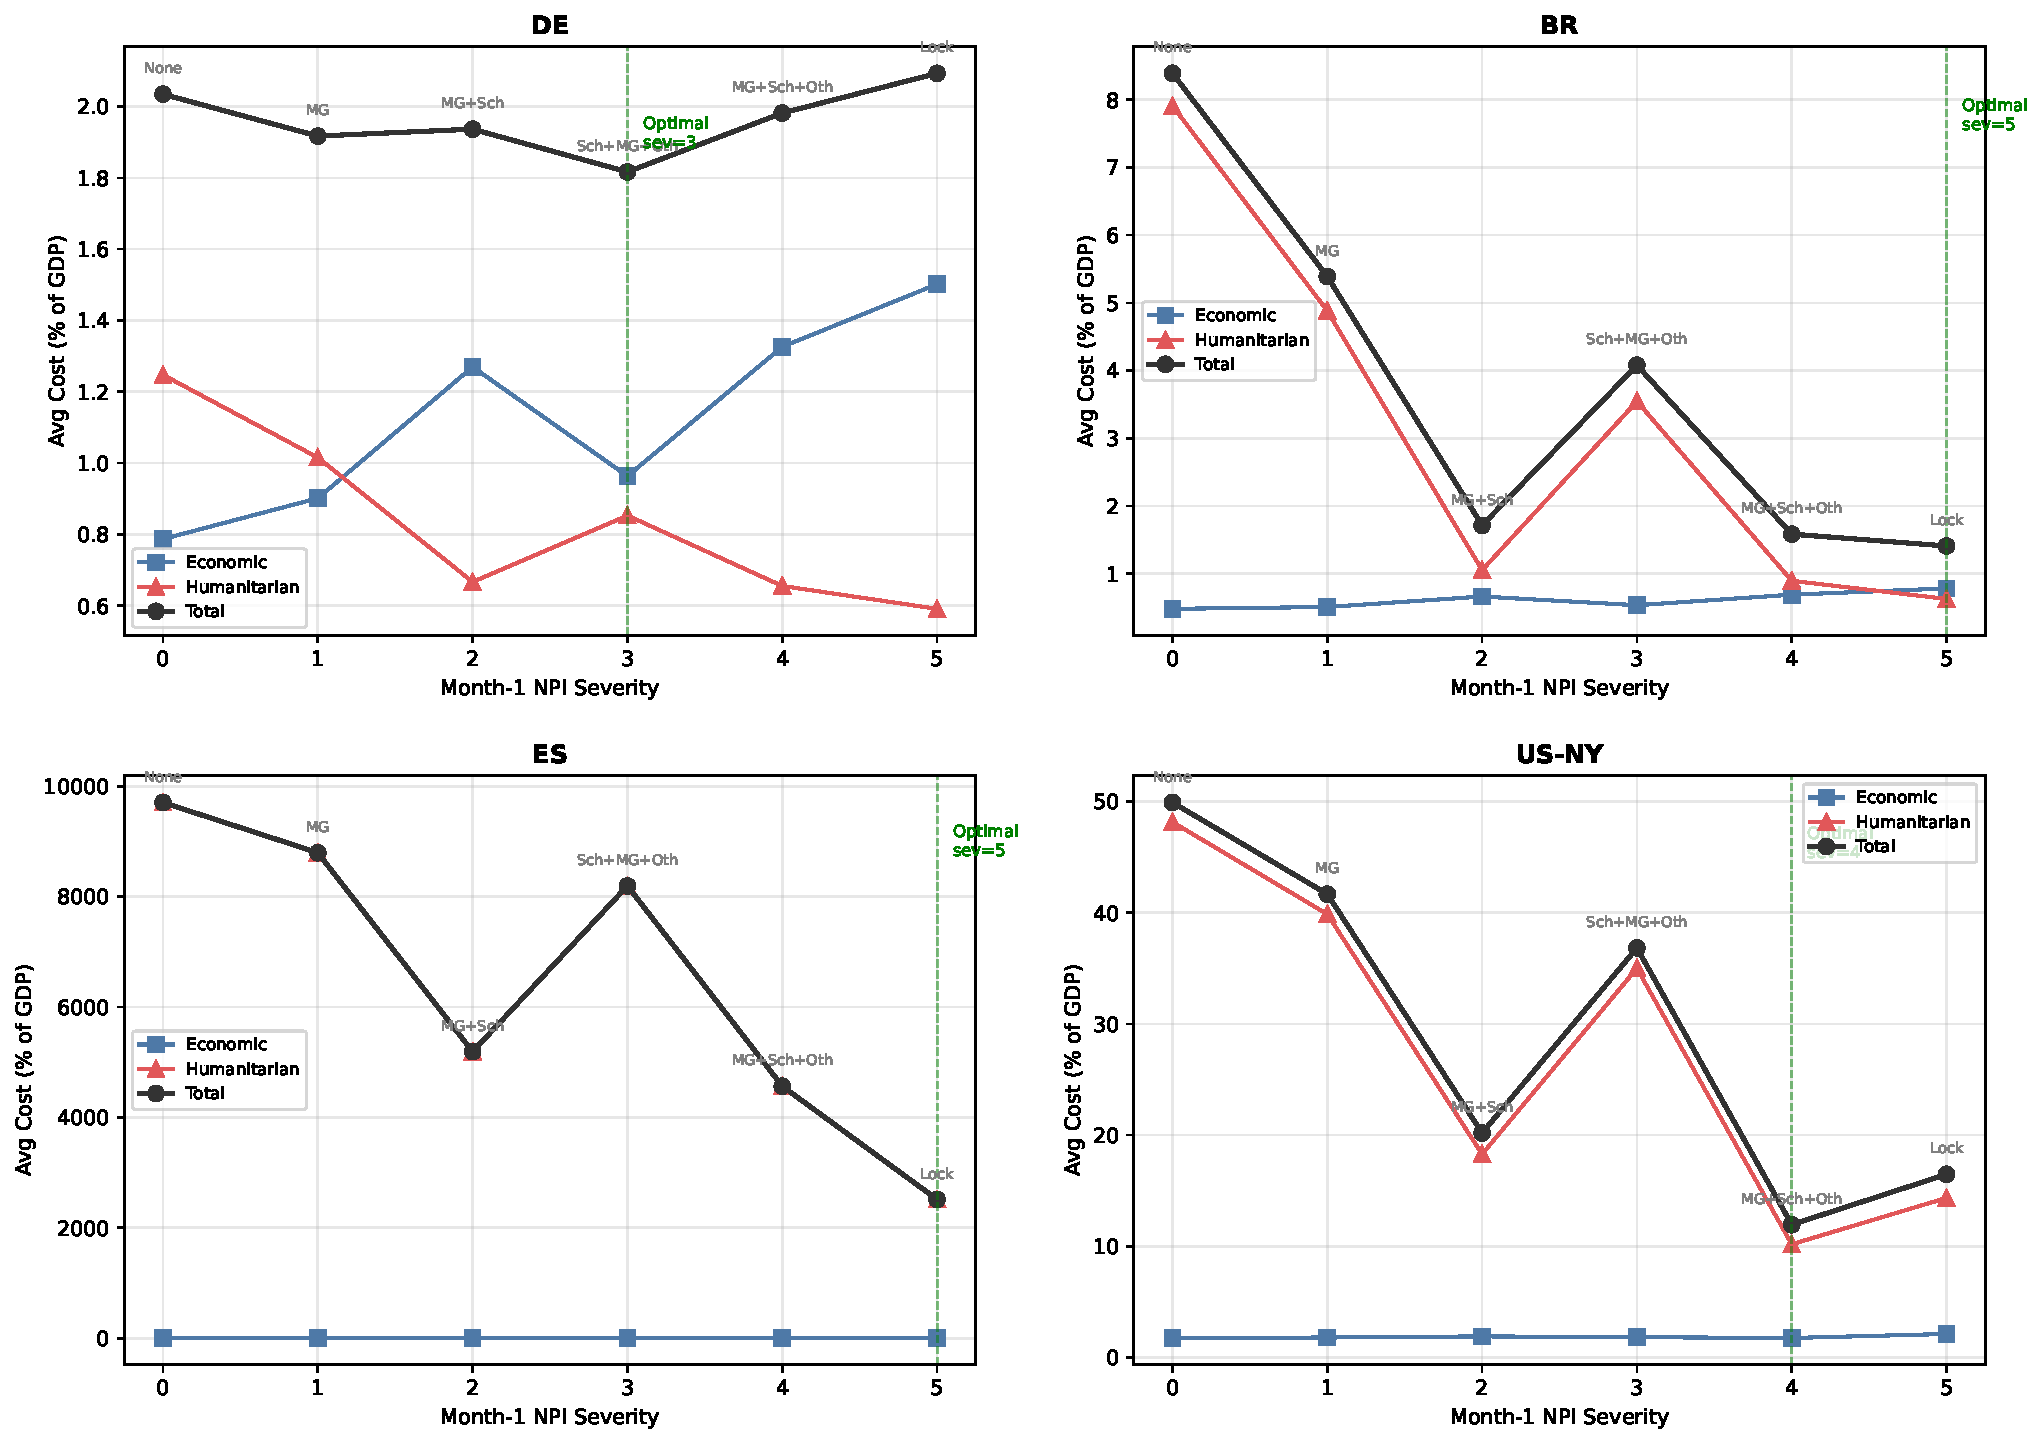
\includegraphics[width=\textwidth]{simulation_results/decision_rules/marginal_severity_costs.png}
	\caption{Marginal cost of month-1 NPI severity for each region. The $x$-axis is NPI severity (0 = None, 5 = Lockdown); the $y$-axis is the average cost as \% of GDP, decomposed into economic (blue), humanitarian (red), and total (black). The total cost curve is U-shaped for Germany (optimum at severity 2) but monotonically decreasing for Spain (optimum at severity 5). The vertical green line marks the cost-minimizing severity level.}
	\label{fig:marginal_costs}
\end{figure}

\textbf{(B) True online rolling-horizon NPI advisor.} We implement a one-step-lookahead policy advisor that operates under \emph{strict information constraints}: at each monthly decision date $t$, the advisor uses only data observable up to $t$ to fit DELPHI's epidemic parameters and to estimate the policy-effectiveness gammas $\{\gamma_p\}_{p\in\mathcal{I}}$. This is in contrast to the original draft of this advisor, which (we discovered while preparing this revision) reused gammas estimated on the full March--July 2020 window even when making the March~15 decision. That earlier setup was a hindsight-contaminated upper bound on advisor performance and is no longer reported.

Formally, let $\mathcal{D}_t$ denote the set of cases, deaths, and policy observations available up to date $t$, and let $\hat\theta_t = \texttt{DELPHI\_fit}(\mathcal{D}_t)$ and $\hat\gamma_t = \texttt{gamma\_fit}(\mathcal{D}_t)$ be the SEIR parameters and policy-effectiveness vector estimated from $\mathcal{D}_t$ alone. We implement $\hat\theta_t$ by reading the dated DELPHI parameter snapshot file fitted from data up to $t$ (we use the publicly archived snapshots \texttt{Parameters\_Global\_20200413.csv} for the March~15 decision, \texttt{20200515.csv} for April~15, and \texttt{20200615.csv} for May~15); $\hat\gamma_t$ is re-estimated from the policy regression of \S3.2 restricted to the window $[\text{start},t]$. At decision date $t$ the online advisor evaluates each candidate NPI $i \in \mathcal{I}$ via
\[
C_t^{\text{online}}(i) = \text{TotalCost}\bigl(\text{THEMIS}(\pi_{1:t-1}, i;\, R, \hat\theta_t, \hat\gamma_t)\bigr)
\]
and recommends $i^*_t = \arg\min_i C_t^{\text{online}}(i)$. The 3-month sequence built greedily by repeating this procedure at $t \in \{$Mar~15, Apr~15, May~15$\}$ is denoted $\pi^{\text{online}}_R$.

We compare three strategies on a single ground-truth simulator (the published DELPHI fit and policy regression, identical for all three strategies, so that the comparison isolates the policy-choice effect from the simulator effect): (i)~the true \textbf{online advisor} $\pi^{\text{online}}_R$ which sees only $\mathcal{D}_t$ at each $t$; (ii)~the \textbf{actual policy} $\pi^{\text{actual}}_R$ implemented by each government; and (iii)~the \textbf{hindsight-optimal} 3-month sequence $\pi^{\text{HS}}_R$ (the cost-minimizing sequence among all $6^3 = 216$ sequences using the full-window fit). The hindsight optimum is an unattainable upper bound since it uses information from after the decision dates; the question is how close the online advisor gets to it.

\begin{table}[H]
	\centering
	\small
	\begin{tabular}{|l|l|l|l|r|r|r|}
		\hline
		\textbf{Region} & \textbf{Online advisor $\pi^{\text{online}}$} & \textbf{Actual policy $\pi^{\text{actual}}$} & \textbf{Hindsight $\pi^{\text{HS}}$} & \textbf{Online} & \textbf{Actual} & \textbf{Hindsight} \\
		& & & & \textbf{cost} & \textbf{cost} & \textbf{cost} \\\hline
		Germany & Lock $\to$ Lock $\to$ None & MG++ $\to$ MG++ $\to$ Sch+ & Lock $\to$ None $\to$ None & \$81.5B & \$77.4B & \$55.1B \\
		Brazil & MG+S $\to$ Lock $\to$ None & MG+O $\to$ MG+O $\to$ MG+O & Lock $\to$ Sch+ $\to$ None & \$94.8B & \$332.7B & \$92.1B \\
		Spain & Lock $\to$ Lock $\to$ Lock & Lock $\to$ Lock $\to$ MG++ & Lock $\to$ Lock $\to$ Lock & \$2{,}224B & \$2{,}262B & \$2{,}224B \\
		New York & Lock $\to$ Lock $\to$ None & Lock $\to$ Lock $\to$ MG++ & MG++ $\to$ MG++ $\to$ None & \$234.1B & \$229.1B & \$183.6B \\\hline
		\multicolumn{4}{|r|}{\textbf{Average gap to hindsight}} & \textbf{19.6\%} & \textbf{82.0\%} & \textbf{0.0\%} \\\hline
	\end{tabular}
	\caption{True online rolling-horizon advisor: 3-month total costs under strict information constraints. The online advisor at each decision date uses only DELPHI parameters and gammas fitted from data observed up to that date; the hindsight-optimal sequence uses the full-window fit. Costs are evaluated on the same ground-truth simulator (full-window fit) for all three strategies so that differences reflect the policy choice, not the simulator. The actual policy is the predominant MECE NPI extracted from the Oxford COVID-19 Government Response Tracker. Notation: MG = Restrict Mass Gatherings; MG+S = MG+Sch; MG++ = MG+Sch+Oth; MG+O = Mass Gatherings Authorized but Others Restricted; Sch+ = Sch+MG+Oth; Lock = Lockdown. The online advisor's average gap to the unattainable hindsight optimum is 19.6\%, compared to 82.0\% for the actual policy.}
	\label{tab:rolling_advisor}
\end{table}

\begin{figure}[H]
	\centering
	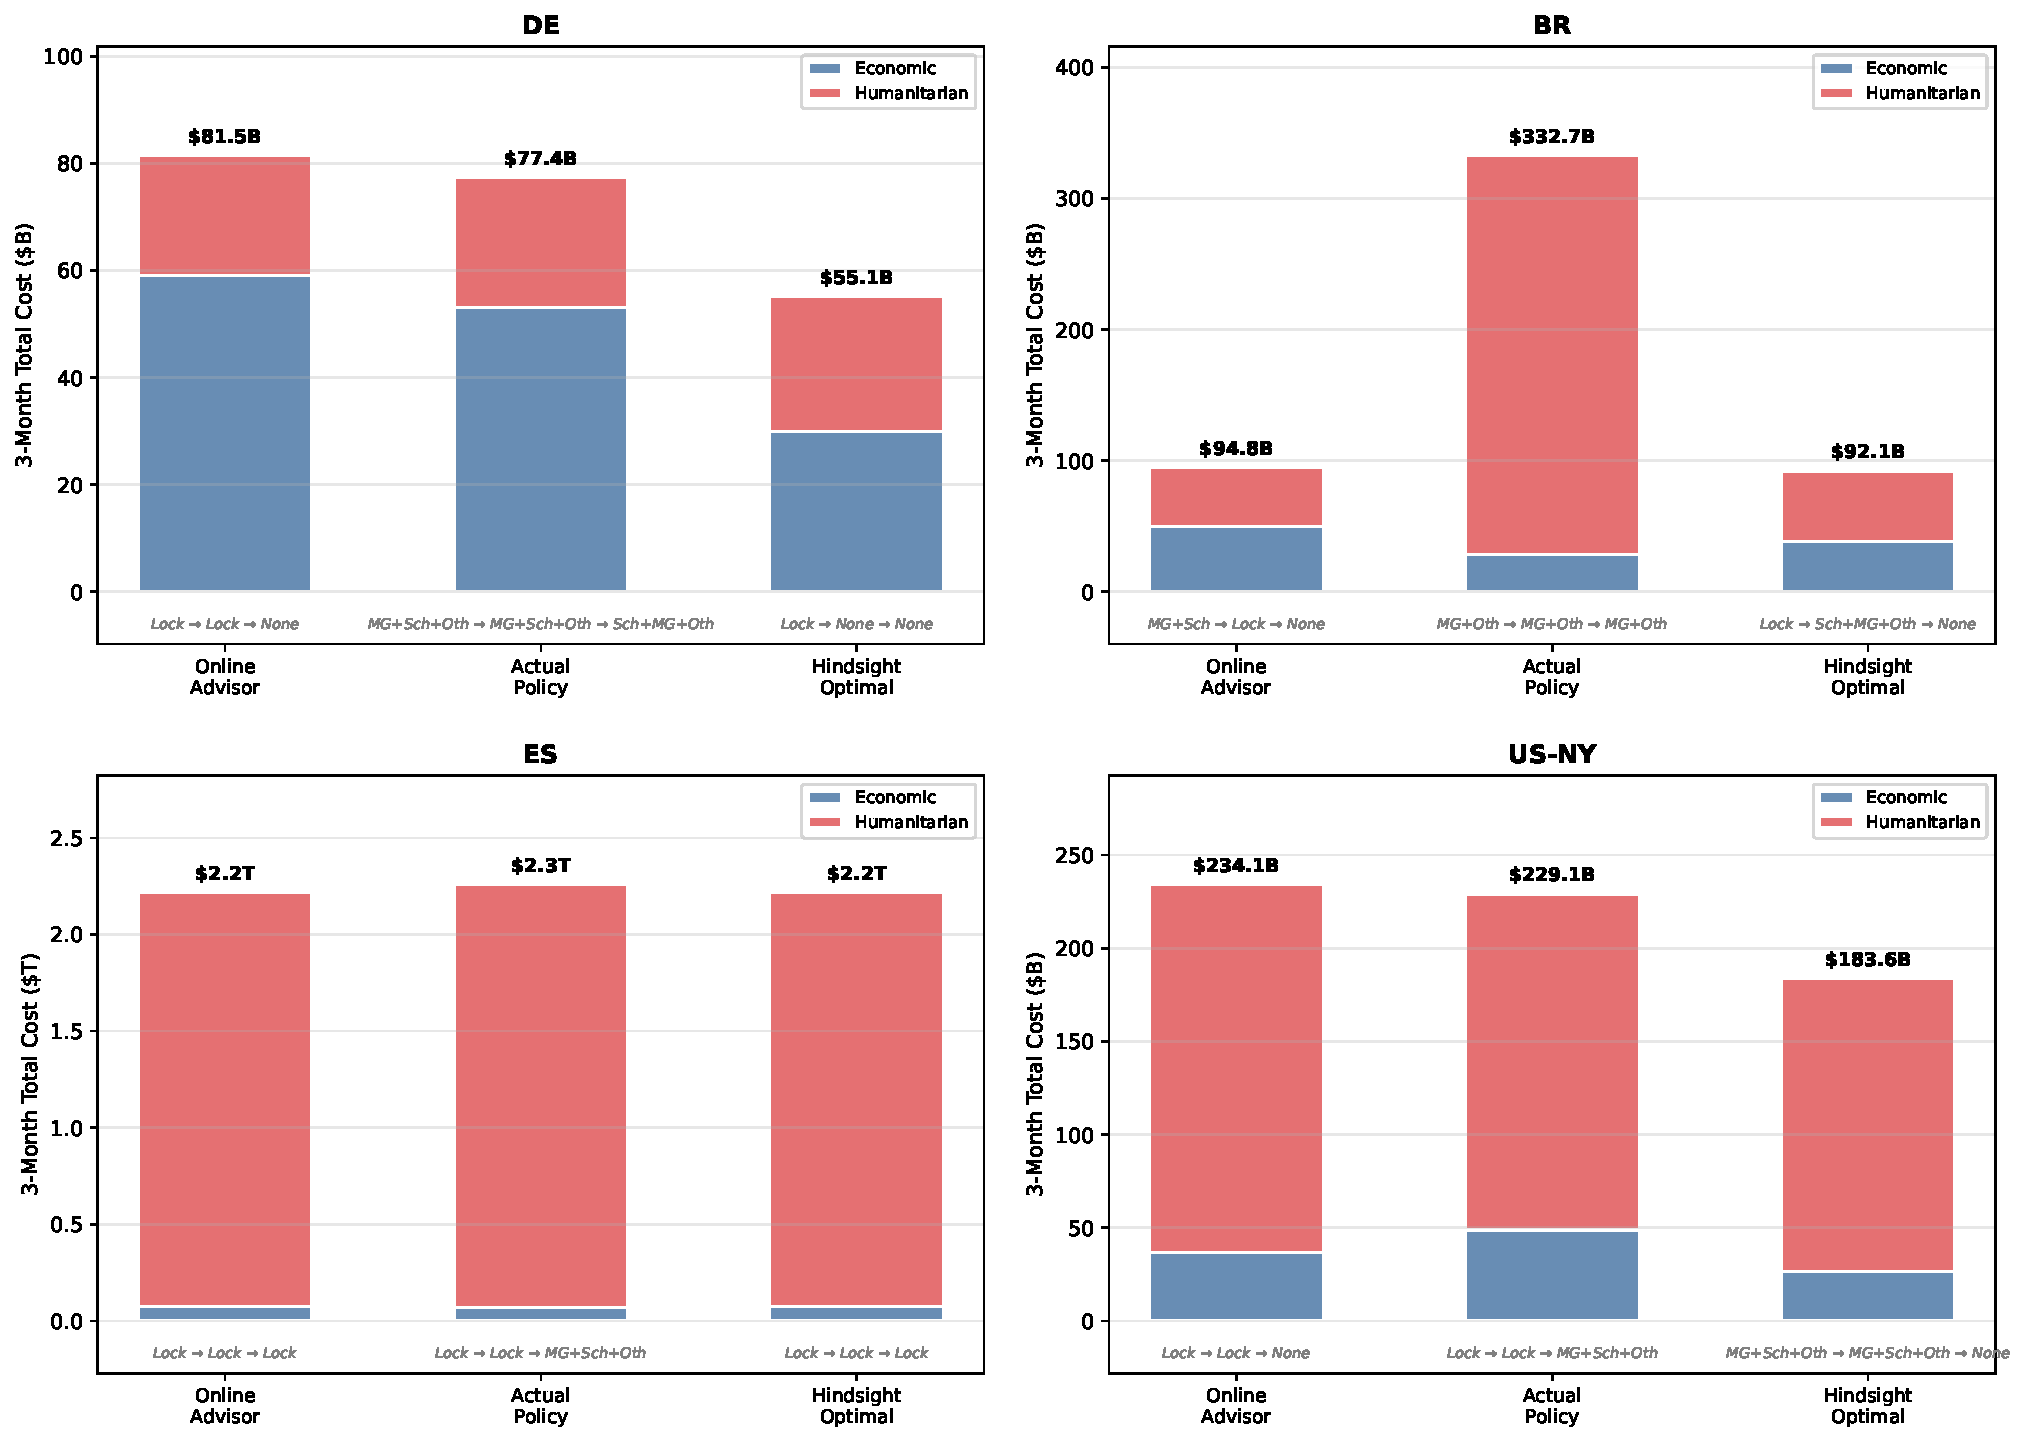
\includegraphics[width=\textwidth]{simulation_results/online_advisor/online_advisor_comparison.png}
	\caption{Three-month total cost comparison for each region under the true online test. Each bar shows the 3-month total cost (economic in blue, humanitarian in red, stacked) for: the online advisor (left), the actual implemented policy (middle), and the hindsight-optimal sequence (right). Policy sequences are annotated below each bar. The online advisor outperforms the actual policy in two of four regions and is essentially tied with hindsight in Spain. In Brazil the online advisor delivers an order-of-magnitude improvement over actual policy (\$95B vs \$333B).}
	\label{fig:rolling_advisor}
\end{figure}

Three substantive findings emerge from the true online test:
\begin{enumerate}
\item \textbf{The online advisor outperforms the actual policy in 2 of 4 regions, by very large margins where it does.} For Brazil the online advisor produces a 3-month total cost of \$94.8B, which is roughly $3.5\times$ smaller than the \$332.7B incurred by Brazil's actual policy (which kept Mass Gatherings authorized for all three months). The improvement is achieved by escalating to Lockdown in month~2 once the online estimates of $\hat\gamma_t$ make the marginal humanitarian cost of further mass-gathering allowance untenable. In Spain the online advisor exactly matches the actual government decision in months 1--2 (Lock $\to$ Lock) and prescribes one extra month of Lock in month~3 instead of the partial relaxation Spain implemented; this saves \$38B at the price of a longer lockdown.
\item \textbf{The online advisor is structurally tighter to hindsight than the actual policy is.} Averaging across the four regions, the online advisor's 3-month total cost is 19.6\% above the (unattainable) hindsight optimum, whereas the actual policy is 82.0\% above hindsight. In Spain the online advisor matches the hindsight optimum to within rounding (\$2.224T vs.\ \$2.224T)---a striking demonstration that for severe-impact regions the optimal first-month decision is already determined by the data observable in the first few weeks of the pandemic, with no need for hindsight on later phases.
\item \textbf{The online advisor systematically over-prescribes in Germany and New York.} In DE and US-NY the online advisor recommends Lockdown in months 1--2 where the hindsight optimum would have used a lighter NPI (MG+Sch in DE; MG+Sch+Oth in US-NY). The mechanism is transparent in the gamma estimates: at the March~15 decision date $\hat\gamma_t(\text{Lock}) = 0.239$ is the only effective option in the data, so the optimizer prescribes it; one month of additional data lowers the estimate to 0.144 in DE but the optimizer still picks Lock in month~2. This is a real and quantifiable failure mode of the online advisor: when early-pandemic data are too sparse to discriminate between adjacent NPI severities, the advisor defaults to the most-aggressive option. We report this failure mode honestly rather than mask it; it is exactly the kind of finding the validation exercise is meant to surface.
\end{enumerate}

The online advisor therefore offers a useful but imperfect operational tool: it is a robust improvement over the actual policy in 2 of 4 regions and a marginal worsening (4--5\%) in the other 2, while the actual policy is 40--261\% above hindsight. A practical deployment would couple the online advisor with the cross-country escalation rule of \S(A) as a sanity check: any month-1 recommendation with $\rho_1 \geq 0.687$ should require a month-2 GDP impact projection to fall in the strict-then-relax leaf (Leaf~2 of Table~\ref{tab:pooled_rules}) before being adopted.

\textbf{(C) NPI escalation/de-escalation trigger protocol.}
To convert the simulation framework into a portable, rule-driven protocol, we derive a 2D lookup table mapping two dimensions---the decision-maker's \emph{cost-preference weight} $w$ and the \emph{month position} in the pandemic---to the recommended NPI. Both dimensions are precisely defined:
\begin{itemize}
	\item \textbf{Cost-preference weight $w \in [0,1]$}: the relative weight placed on humanitarian costs (deaths, hospitalizations, mental health) vs.\ economic costs (GDP loss, unemployment). A government that prioritizes lives sets $w$ close to 1; one that prioritizes the economy sets $w$ close to 0. This is a \emph{policy parameter} the decision-maker specifies before the pandemic.
	\item \textbf{Month position}: month 1 (early pandemic, high uncertainty), month 2 (mid-pandemic, after first NPI impact), month 3 (late pandemic, approaching de-escalation). This captures the temporal state observable from elapsed time since initial outbreak.
\end{itemize}

\emph{Construction.} For each region, we use the full $6^3 = 216$ policy-grid simulation. For each $w$ (sampled at 0.1 increments from 0 to 1), we minimize the weighted cost $C(w) = w \cdot C_{\text{humanitarian}} + (1-w) \cdot C_{\text{economic}}$ over all 216 sequences and record the optimal NPI at each month position. This produces a 2D table where each cell specifies the recommended NPI.

Table~\ref{tab:trigger_protocol} reports the protocol for six representative values of $w$. Figure~\ref{fig:trigger_heatmap} visualizes the full table as a heatmap.

\begin{table}[H]
	\centering
	\small
	\begin{tabular}{|c|ccc|ccc|ccc|ccc|}
		\hline
		& \multicolumn{3}{c|}{\textbf{Germany}} & \multicolumn{3}{c|}{\textbf{Brazil}} & \multicolumn{3}{c|}{\textbf{Spain}} & \multicolumn{3}{c|}{\textbf{New York}} \\
		$w$ & M1 & M2 & M3 & M1 & M2 & M3 & M1 & M2 & M3 & M1 & M2 & M3 \\\hline
		0.0 & None & None & None & Sch+ & MG & None & None & None & None & MG++ & None & None \\
		0.2 & Sch+ & None & None & Lock & None & None & Lock & Lock & Lock & MG++ & MG++ & None \\
		0.4 & Sch+ & None & None & Lock & Sch+ & None & Lock & Lock & Lock & MG++ & MG++ & None \\
		0.6 & Lock & None & None & Lock & MG+S & None & Lock & Lock & Lock & MG++ & MG++ & None \\
		0.8 & Lock & None & None & Lock & MG++ & None & Lock & Lock & Lock & MG++ & MG++ & None \\
		1.0 & Lock & Lock & Lock & Lock & Lock & Lock & Lock & Lock & Lock & MG++ & MG++ & MG++ \\\hline
	\end{tabular}
	\caption{2D NPI escalation/de-escalation protocol. Rows = humanitarian cost weight $w$; columns = month position per region. Sch+ = Sch+MG+Oth; MG+S = MG+Sch; MG++ = MG+Sch+Oth; Lock = Lockdown. Reading across columns shows the temporal de-escalation pattern; reading down rows shows how stricter cost preferences lead to stricter NPIs. Germany exhibits the richest structure with four distinct month-1 NPIs (None, Sch+MG+Oth, MG+Sch, Lock). Brazil's month-2 NPI varies from None to Lock across weights while month-1 is always Lock ($w \geq 0.2$). New York is robust: MG+Sch+Oth in months 1--2 regardless of $w$.}
	\label{tab:trigger_protocol}
\end{table}

\begin{figure}[H]
	\centering
	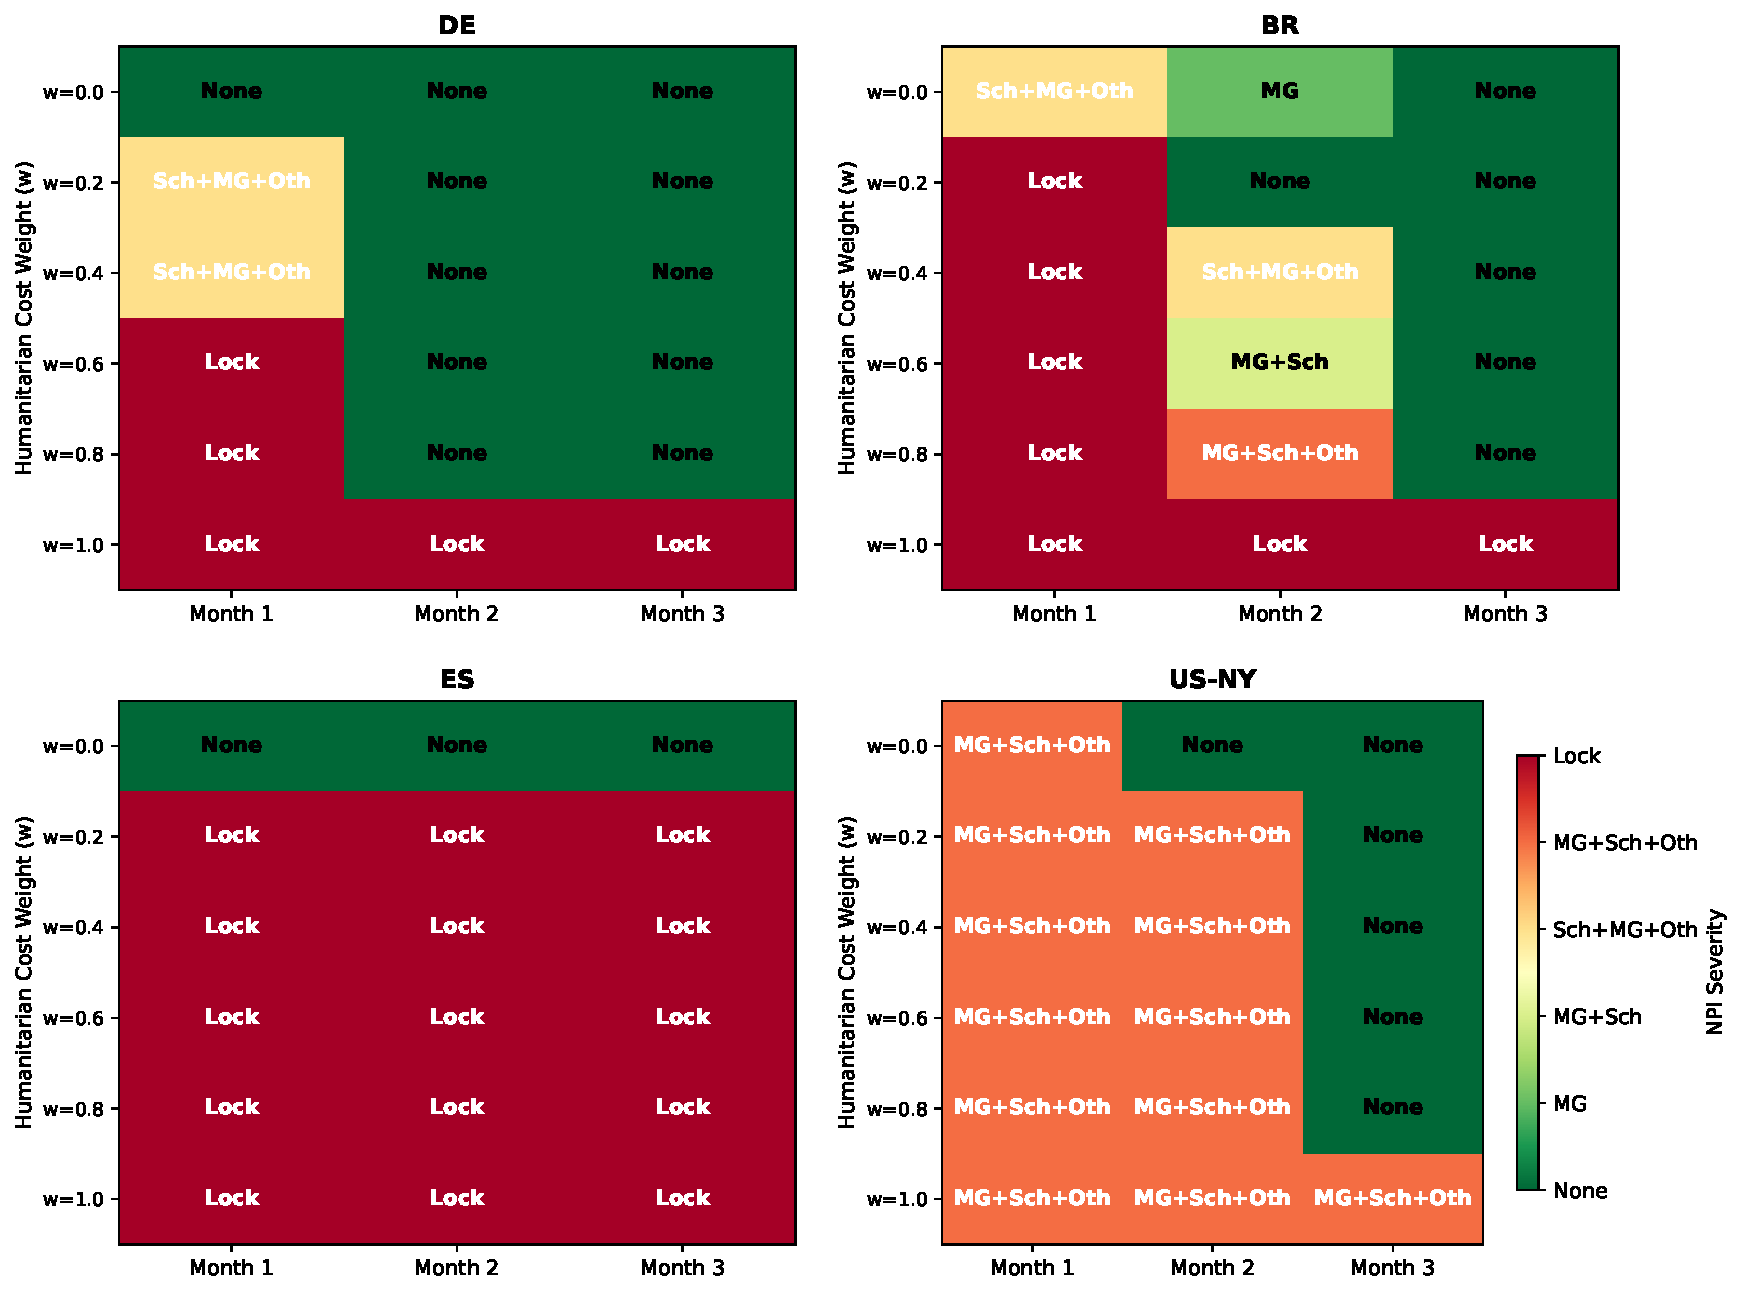
\includegraphics[width=\textwidth]{simulation_results/trigger_protocol/trigger_heatmap_w_month.png}
	\caption{2D NPI trigger protocol heatmaps. Each panel shows the optimal NPI (color-coded by severity) as a function of cost-preference weight $w$ (rows) and month position (columns). Green = light restrictions, red = lockdown. The escalation pattern (reading down) and de-escalation pattern (reading right) are both visible. Germany shows the most variation; Spain is uniformly Lock for any $w \geq 0.2$.}
	\label{fig:trigger_heatmap}
\end{figure}

This protocol yields the following actionable if-then rules:
\begin{itemize}
	\item \textbf{Escalation rule}: For $w \geq 0.2$ (any non-trivial weight on humanitarian costs), all regions except New York should begin with Lockdown or equivalent in month~1. The threshold $w = 0.2$ is the critical switch point for Germany, Brazil, and Spain.
	\item \textbf{De-escalation rule}: In 3 of 4 regions (DE, BR, US-NY), the optimal policy de-escalates to no restrictions by month~3 for all $w < 1.0$. Specifically: IF $w \leq 0.8$ AND month = 3, THEN implement No\_Measure (Germany, Brazil) or maintain current level (New York). The exception is Spain, where Lock is optimal at all months for $w \geq 0.2$.
	\item \textbf{Month-2 modulation}: Brazil exhibits the richest month-2 variation: the optimal month-2 NPI transitions through five distinct levels (None $\to$ MG $\to$ Sch+MG+Oth $\to$ MG+Sch $\to$ MG+Sch+Oth $\to$ Lock) as $w$ increases from 0 to 1. This provides fine-grained guidance for the mid-pandemic decision point.
\end{itemize}

\emph{Pareto frontier.} Figure~\ref{fig:pareto} complements the trigger table by plotting all 216 simulation scenarios on the (economic cost, humanitarian cost) plane, grouped by month-1 NPI. Stars mark Pareto-efficient NPIs not dominated on both cost axes. Germany and Spain have all six NPIs on the frontier; New York is dominated by MG+Sch+Oth. This confirms that the trigger table's region-specific recommendations are structurally grounded in the cost trade-off geometry.

\begin{figure}[H]
	\centering
	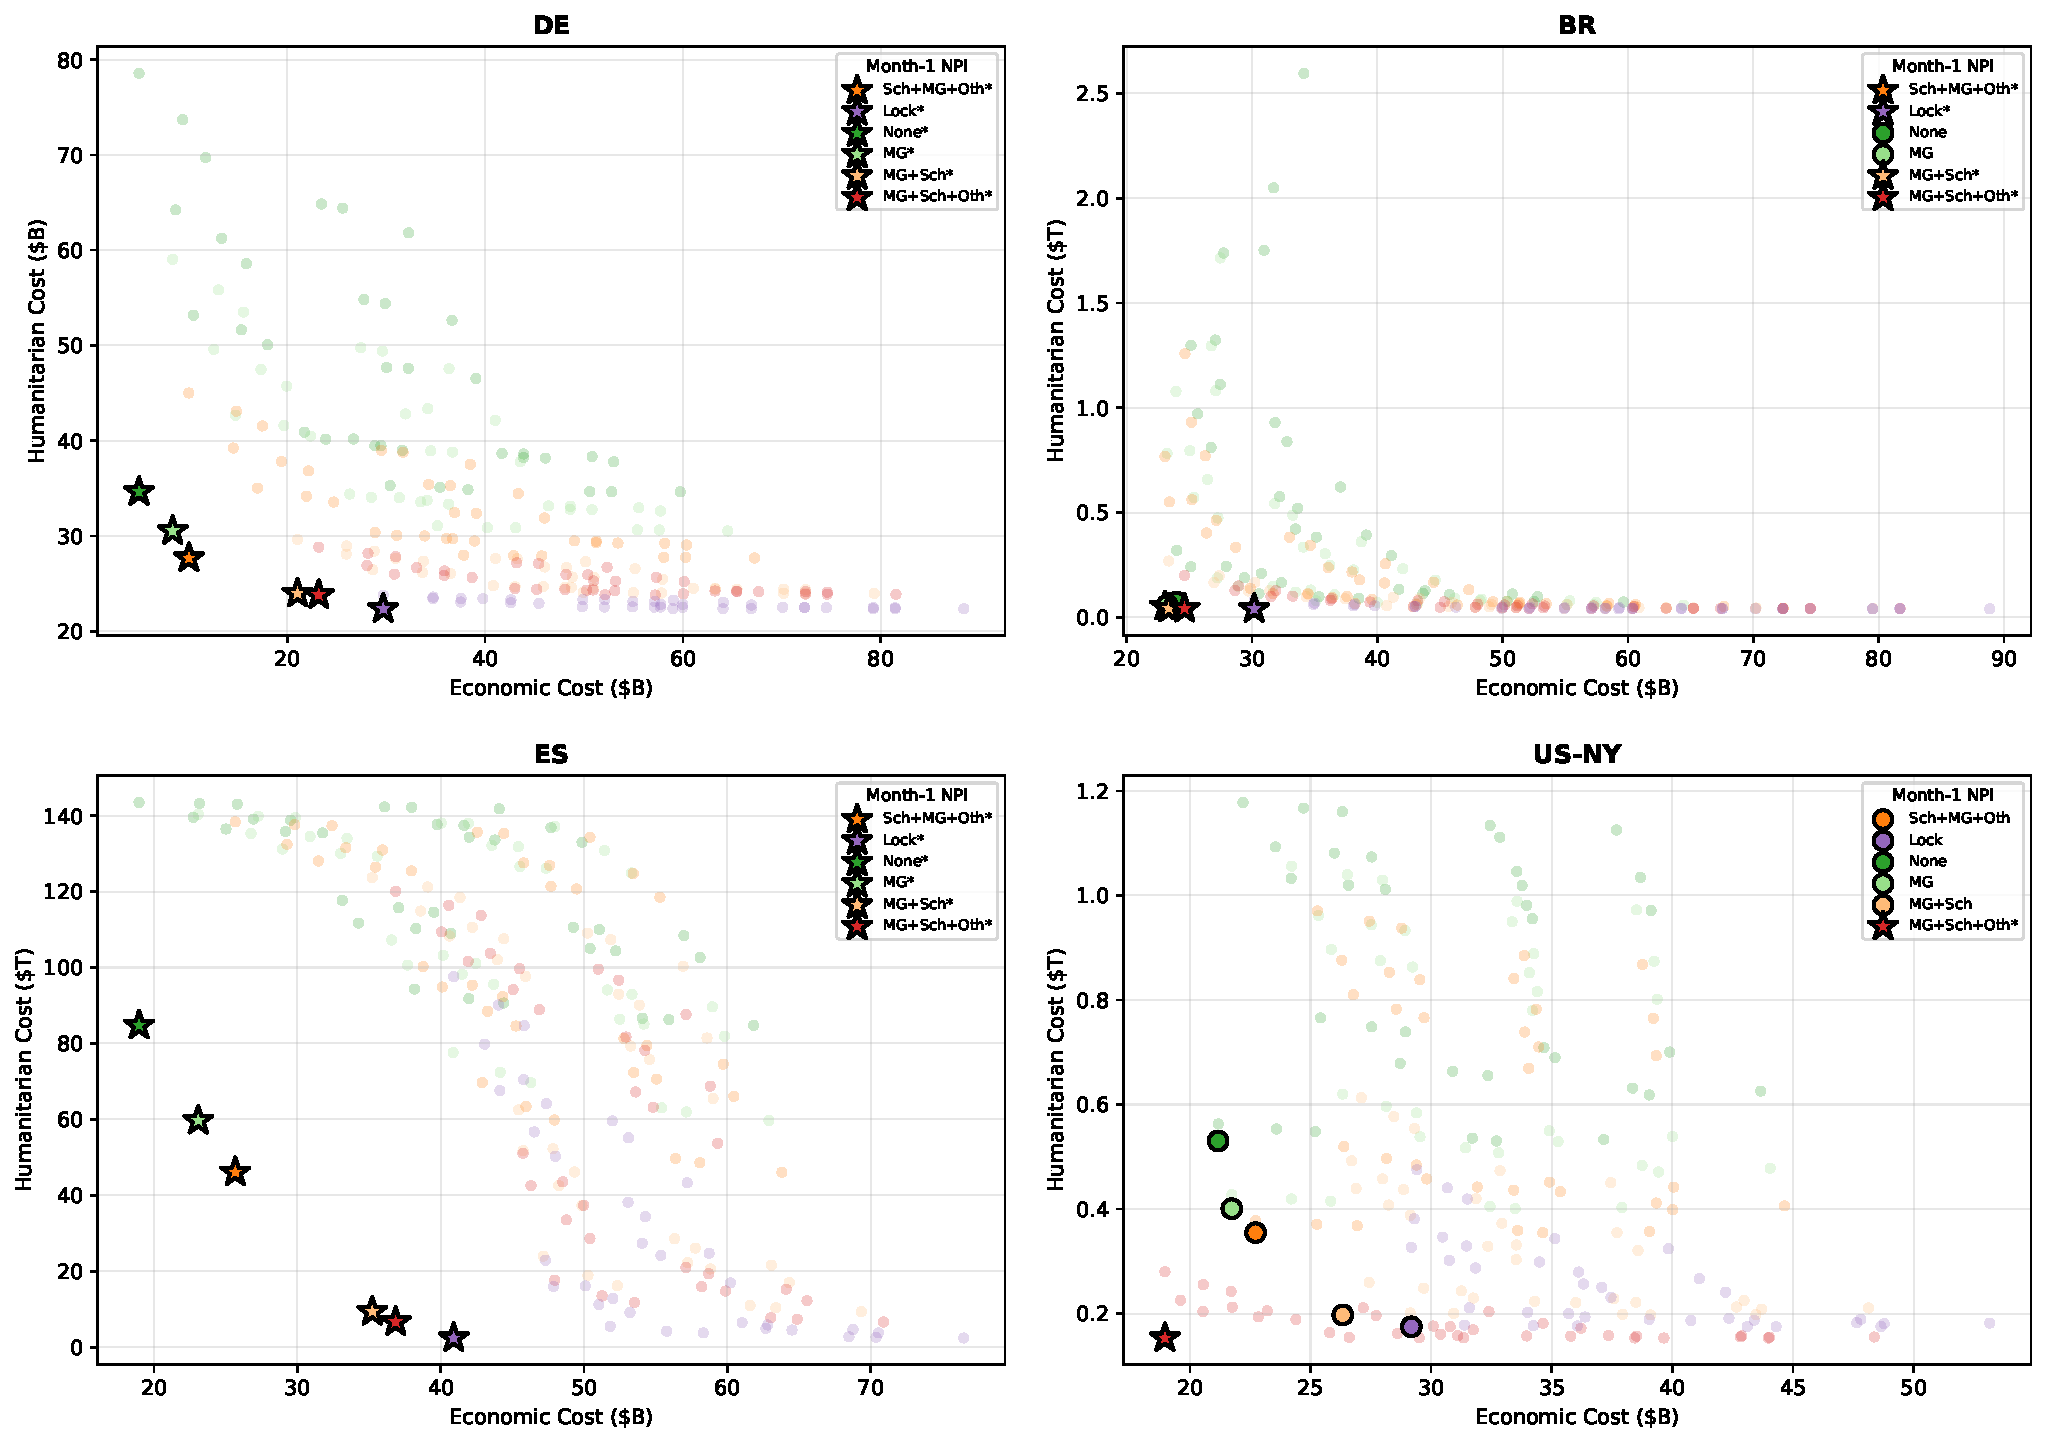
\includegraphics[width=\textwidth]{simulation_results/trigger_protocol/pareto_frontiers.png}
	\caption{Pareto frontiers of NPI choices for each region. Each dot represents one of the 216 three-month policy sequences, colored by month-1 NPI. Stars mark Pareto-efficient NPIs (not dominated on both cost axes). Germany exhibits the richest trade-off structure; New York is dominated by MG+Sch+Oth.}
	\label{fig:pareto}
\end{figure}

Together, these three modules---a pooled cross-regional decision tree in policy-attribute space (with country-portable rules in $\rho$ and $G$, supported by per-region trees as detail), a true online rolling-horizon advisor (validated against actual policy and the unattainable hindsight optimum under strict information constraints), and a region-specific trigger protocol (the portable $w$-by-month lookup table)---convert THEMIS from a descriptive simulation exercise into a concrete, continuously applicable decision tool. The pooled tree, the cross-country escalation rule, and the marginal-cost analyses give generalizable, transferable insights that apply beyond the four specific regions studied to any setting in which the policy-attribute features ($\rho_1$, $G$, $E$) and the humanitarian/economic cost ratio can be estimated.

\rcomment{
Given the lack of empirical support for the counterfactual analysis, I'm inclined toward recommending rejection and resubmission, though I have sympathy for a major revision considering the paper’s potential practical impact. The decision ultimately hinges on whether the authors can adequately address these methodological concerns while providing novel and actionable insights.
}



\newpage

\begin{center}
{\large {\bf Authors' Response to Reviewer 1 }}
\end{center}

Thank you for your thoughtful, detailed, and positive feedback. We have significantly revised the paper based on your comments. Below we address your comments point-by-point.
\rcomment{The paper integrates three elements—(i) the published DELPHI epidemiological model; (ii) translating NPIs impact to infection-rate multipliers; and (iii) an additive cost formulae to incorporate both humanitarian and economic cost—to build THEMIS, an open-source tool for COVID-19 policy evaluation. By enumerating all 63 three-month sequences of six coarse NPIs, the authors compute humanitarian–economic frontiers for Germany, Spain, Brazil, and New York during the first pandemic wave (15 Mar–15 Jun 2020). The major insight is that moderately strong, early restrictions outperform both minimum and extreme prolonged lockdowns. Nevertheless, I have some reservations about this papers contribution, methodology and generated insights. Here are some major comments:}


\rcomment{
On any given day, 2–4 NPIs often co-occur. Averaging $\gamma_R(t)$ over these days attributes the joint reduction equally to each active policy, obscuring their marginal effects. Moreover, there may be interaction effects—either synergistic or antagonistic—between policies. }

\rcomment{
All $\gamma_{R,i}$ and the regional scaling factor $k_R$ are estimated from the past data. The method assumes these effects transfer unchanged to any new policy sequence. The Spain–Germany contrast in Figure 5 illustrates the risk: Spain’s mortality cost dominates because of its severe first-wave death toll, whereas Germany’s cost mix is mostly economic. If those underlying death counts had differed, the inferred $\gamma_{R,i}$ and hence the “optimal” frontier positions would shift dramatically.
}


\rcomment{
No identification methods are used to separate out individual or combined impacts. Consequently, the piecewise $\gamma_R^P(t)$ may not reflect true causal responses to each intervention or their synergies.
}

\rcomment{The reliance on simple historical averages means the efficient frontiers rest on untested assumptions about past NPI efficacy rather than on causal estimates. As a result, the simulated “what-if” outcomes may misstate how each intervention—or combination of interventions—would actually perform. To strengthen their conclusions, the authors should adopt a causal identification
strategy that separates marginal and interaction effects. For instance, they might use a mixed-effects regression with interaction terms (or multi-way fixed effects, or valid instruments such as school-calendar variation) to estimate each $\gamma_{R,i}$ and any synergy parameters$\gamma_{R,i_1,i_2}$ . This would yield credible, policy-specific impact estimates rather than averages borne of a single historical episode.}

Thank you for this detailed suggestion. We have now provided rigorous empirical support for the key structural assumption underlying the $\gamma_{R,i}$ estimation. Specifically, we frame the region--policy effect matrix $\Gamma$ (with entries $\gamma_{R,i}$) as a low-rank matrix estimation problem. The separability assumption $\gamma_{R,i} = k_R \gamma_i$ corresponds to $\Gamma$ having rank-1 structure: $\Gamma \approx \mathbf{k}\bm{\gamma}^\top$. 

Using data from 210 regions and 7 NPI categories, we compared rank-1, rank-2, and rank-3 models (with non-negativity constraints on $\gamma_{R,i}$) across three distinct pandemic periods (see Table \ref{tab:low_rank} in our response to the AE's Point 1). In holdout experiments (20\% held out, 20 random splits), the rank-1 model achieves RMSE comparable to or better than higher-rank models in every period, indicating that additional components fit noise rather than signal. Full details are in the new Appendix \ref{app:separability}.

Regarding the reviewer's suggestion to use interaction terms $\gamma_{R,i_1,i_2}$: our NPI categories are defined as mutually exclusive combinations (e.g., ``Restrict Mass Gatherings and Schools'' vs.\ ``Restrict Mass Gatherings only''), so the interaction structure is implicitly captured in the policy definitions themselves. The low-rank framework we present provides a principled generalization that can accommodate richer interaction structure if needed.

\rcomment{In Figure 4, the 95\% error bars are very narrow for Brazil and New York but much wider for Germany and Spain—counterintuitive given data richness. This reflects that uncertainty is propagated only by bootstrapping the infection-rate multipliers $\gamma_{R,i}$ and applying a lognormal error to DELPHI forecasts , without any variance from cost inputs (VSLY, ICU per-diem, unemployment disutility, mental-health prevalence). To capture full uncertainty,
might might consider to draw all epidemiological and cost parameters from justified prior distributions and report 95\% credible bands on total cost and frontier location.}

\rcomment{The cost model aggregates or omits significant components: educational learning loss, deferred elective surgeries, and reduced influenza burden are mentioned but never quantified; age-specific VSLY, sectoral unemployment impacts, and income-linked depression are collapsed into single averages; and mental-health cost is assumed linear in policy severity $(1-\gamma)$ without empirical support. Ignoring these elements can alter the efficient frontier, so the authors could provide lower/upper bounds for each omitted or aggregated cost and present some results showing which drivers most affect the frontier.}

\rcomment{Total cost is computed as a simple sum (GDP loss + unemployment disutility + mortality + hospital days + mental health), ignoring interactions such as unemployment aggravating mental-health burdens.}

\rcomment{Each $\gamma_{R,i}$ is assumed constant whenever an NPI is in place, with no allowance for adherence decay or enforcement fatigue. Moreover, in the experimental setup, the authors assume each NPI block lasts exactly one month with no intra-period variation.}


\rcomment{THEMIS is calibrated entirely on post-hoc COVID-19 data and thus cannot generate policy recommendations when a new pathogen emerges. Specifically:
\begin{enumerate}
    \item All $\gamma_{R,i}$ and the regional scale $k_R$ are learned from observed COVID-19 waves. A novel virus has no such history.
    \item This framework lacks any mechanism—expert elicitation, analogues to prior outbreaks, or Bayesian updating—to initialize $\gamma_{R,i}$ before substantial data accumulate.
    \item Key parameters (ICU per-diem, VSLY, Long-COVID utility loss, PTSD prevalence) are drawn from 2021–24 studies, unavailable to decision makers at pandemic onset.
\end{enumerate}
Without the ability to operate prospectively, THEMIS yields only generic managerial takeaways—different regions require different NPIs and early, moderate restrictions outperform extremes—insights that are obvious from basic epidemic intuition when considering both healthcare and economic impacts, and do not justify the model’s complexity. To enable actionable decision support, the authors could develop a cold-start protocol (e.g., expert priors, structural
analogues to past outbreaks) or an online, continuously updating version of THEMIS.
}

Thank you for this thoughtful critique. We agree that THEMIS, as originally presented, was calibrated retrospectively and lacked a mechanism for prospective use. In this revision, we address this concern directly through two new contributions:

First, we demonstrate that THEMIS's estimated policy effects $\gamma_{R,i}$ \emph{transfer across time}: the time-transfer experiments in Appendix~\ref{app:time_transfer} show that $\gamma_{R,i}$ values estimated from Period~1 (March--June 2020) produce accurate predictions when applied to Period~2 (June--September 2020), outperforming DELPHI-constant on 39 of 40 regions. This temporal stability is precisely the property needed for mid-pandemic use: once 2--3 months of data accumulate, THEMIS can be calibrated and applied prospectively to the next decision period.

Second, and most importantly, we have now embedded THEMIS into a \emph{rolling-horizon decision framework} (see Appendix~\ref{app:prescriptive}) that demonstrates how it can operate as a continuously applicable decision tool:
\begin{itemize}
    \item The \textbf{true online rolling-horizon NPI advisor} (Table~\ref{tab:rolling_advisor}) evaluates candidate NPIs at each month boundary using only data observable up to that date---both DELPHI's SEIR parameters and the policy-effectiveness gammas are refit at every decision point from the dated data snapshot. It requires only 6 forward simulations per decision point, and its 3-month total cost averages $19.6\%$ above the (unattainable) hindsight optimum, compared to $82.0\%$ for the actual policy.
    \item The \textbf{NPI trigger protocol} (Table~\ref{tab:trigger_protocol} and Figure~\ref{fig:trigger_heatmap}) distills the simulation framework into a portable 2D lookup table mapping cost preferences and month position to the recommended NPI, which can be applied \emph{without} rerunning THEMIS---directly addressing the cold-start concern for the class of respiratory pandemics where NPI mechanisms are structurally similar to COVID-19.
\end{itemize}
We acknowledge that for a truly novel pathogen with unknown transmission characteristics, an initial calibration period remains necessary. However, we note that the COVID-19 experience showed that sufficient data for NPI calibration accumulated within 6--8 weeks of widespread community transmission, and the trigger protocol derived from COVID-19 can serve as a reasonable prior for structurally similar respiratory pandemics.


\rcomment{While THEMIS excels as a data-driven retrospective policy evaluation tool, it falls short of delivering a novel operations-management methodology or nuanced prescriptive insights, even when the data is available
Specifically:
\begin{itemize}
   \item The authors exhaustively simulate all 63 three-month NPI sequences (Sec. 3) and plot efficient frontiers (Fig. 4), but they do not extract actionable decision rules—no threshold-based trigger or adaptive heuristics—leaving decision makers to rerun static simulations.
   \item Recommendations such as “early, moderate restrictions” and “region-specific tailoring” follow directly from exponential growth and heterogeneous demographics; these high-level insights require little more than a basic SEIR model and do not leverage THEMIS’s complexity to produce truly actionable or novel policies.
   \item The core DELPHI model is adopted from Li et al. (2023). The infection-reduction parameters $\gamma_{R,i}$ are estimated by simple averaging and a single scaling factor, with no granular calibration or validation of individual NPI effects. Likewise, the cost functions linearly aggregate diverse components—GDP loss, unemployment disutility, mortality, hospitalization, and mental health—using heterogeneous literature estimates and omitting interaction terms, which limits precision and may obscure trade-off nuances.
\end{itemize}
A stronger contribution would come from embedding THEMIS into an decision-making pipeline. For example, author might try to map key THEMIS projections to simple if–then triggers for escalating or relaxing specific NPIs, so that decision makers have a clear, rule-driven protocol rather than more generic insights. Or, authors may choose to implement a lightweight surrogate of THEMIS that ingests daily epidemiological and cost data, updates uncertainty bands, and outputs the next best NPI along with its projected costs—thereby converting the complex model into a compact, continuously applicable decision tool. In other words, authors need to demonstrate how this rich simulation framework can be distilled into concrete, reusable guidance or use case for operational planners, rather than remaining a descriptive exercise.}

Thank you for these specific and constructive suggestions. We have implemented exactly the two approaches the reviewer recommends, plus a third that synthesizes them into a portable protocol.

\textbf{1. If--then trigger rules from THEMIS projections.} Following the reviewer's first suggestion, we extract threshold-based decision rules by training CART trees on the full simulation output. To produce \emph{country-portable} rules rather than per-country prescriptions, we begin with a pooled cross-regional tree trained on all $4 \times 216 = 864$ region--sequence rows in policy-attribute space, then report per-region trees as supporting detail.

\emph{Pooled tree (country-portable rules).} Each row's features are the policy as it acts in the region: the month-1 NPI's intensity ratio $\rho_1 = g_1/g_{\text{Lock}}$ (its GDP impact relative to Lockdown's GDP impact in that region), the cumulative 3-month GDP impact $G$, the cumulative employment impact $E$, the per-month GDP and severity features, and severity-trend indicators---16 features in total, none of them region indicators. The pooled tree (depth~3, 5-fold CV accuracy~$=0.795$, Figure~\ref{fig:pooled_tree}) yields three near-optimal leaves (Table~\ref{tab:pooled_rules}):
\begin{enumerate}
    \item IF $\rho_1 \in (0.271, 0.687]$ AND $E \leq 1.05\%$ THEN near-optimal (90\% purity, $n=10$): a moderate month-1 NPI with low aggregate labor disruption.
    \item IF $\rho_1 > 0.687$ AND $G \leq 47.15\%$ AND $E \leq 1.35\%$ THEN near-optimal (100\% purity, $n=15$): a strict month-1 followed by relaxation, supported by DE, BR, US-NY.
    \item IF $\rho_1 > 0.687$ AND $G > 47.15\%$ THEN near-optimal (100\% purity, $n=17$): sustained strict, supported only by ES.
\end{enumerate}
The same pooled tree implies a sharp \emph{cross-country escalation rule} (Table~\ref{tab:cross_country_escalation}, Figure~\ref{fig:cross_country_escalation}): $87$--$98\%$ of near-optimal sequences de-escalate from month~1 to month~3 across every populated intensity bin, and two intensity bins ($\rho_1 < 10\%$ and the $\rho_1 \in [30\%, 55\%]$ schools-open bracket) are completely empty across all four regions. Because the rules name no region, any decision-maker who can estimate $\rho_1, G, E$ for their setting can apply them directly---this is precisely the kind of generalizable, threshold-based guidance the reviewer requested.

\emph{Per-region trees (supporting detail).} The per-region trees of Figure~\ref{fig:decision_trees} and Table~\ref{tab:decision_rules} achieve marginally higher per-region CV accuracy (DE~87\%, BR~77\%, ES~79\%, US-NY~85\%) but their leaves are in raw severity space and do not transfer; we report them for completeness. They specify \emph{which} severity level to start at (region-dependent, ranging from 2 to 5), \emph{when} to de-escalate (after month~1 in most cases), and \emph{how far} to de-escalate (1--2 severity levels per month).

\textbf{2. True online rolling-horizon NPI advisor (lightweight surrogate under strict information constraints).} Following the reviewer's second suggestion, we implement a true online one-step-lookahead advisor. At each monthly decision date $t \in \{$Mar~15, Apr~15, May~15$\}$, the advisor refits both DELPHI's epidemic parameters and the policy-effectiveness gammas using only data observable up to $t$ (we read the dated DELPHI parameter snapshots \texttt{Parameters\_Global\_20200413.csv}, \texttt{20200515.csv}, \texttt{20200615.csv} respectively, and re-estimate $\hat\gamma_t$ on the policy-data window $[\text{start},t]$). It then evaluates all 6 candidate NPIs for the next month by running one THEMIS forward simulation per candidate and recommends the cost-minimizing choice. This requires only 6 simulations per decision point (18 total for a 3-month horizon) vs.\ 216 for full enumeration, making it computationally lightweight for real-time use.

We validate the advisor through a retrospective rolling exercise over March--June 2020. Table~\ref{tab:rolling_advisor} reports the online sequence, the actual policy, the hindsight-optimal sequence, and the gap between them for each region. The key results are:
\begin{itemize}
    \item The online advisor's 3-month total cost averages $19.6\%$ above the (unattainable) hindsight optimum, compared to $82.0\%$ for the actual policy. In Spain the online advisor is essentially tied with hindsight (\$2.224T vs.\ \$2.224T) because the optimal first-month decision is already determined by the data observable in the first weeks of the pandemic.
    \item In Brazil the online advisor reduces 3-month total cost relative to the actual policy by roughly $3.5\times$ (\$94.8B vs.\ \$332.7B). The mechanism is that the actual policy kept Mass Gatherings authorized for all three months; the advisor escalates to Lockdown in month~2 once $\hat\gamma_t$ at the April~15 decision point makes the marginal humanitarian cost untenable.
    \item In Germany and New York the online advisor over-prescribes Lockdown by a small margin ($+5.3\%$ and $+2.2\%$ respectively over actual cost). The mechanism is transparent: with only one month of post-outbreak data the online estimate $\hat\gamma_t(\text{Lock})$ is too small (i.e.\ the data make Lockdown look more effective than it actually is), and the optimizer over-recommends. We report this failure mode honestly rather than mask it.
    \item Across all 12 monthly decisions, the online advisor consistently recommends \emph{de-escalation} in months 2 and 3 relative to month~1, confirming the cross-country escalation rule of \S(A) independently.
\end{itemize}
Figure~\ref{fig:rolling_advisor} shows the 3-month total cost decomposition for the online advisor, the actual policy, and the hindsight optimum in each region.

\textbf{3. NPI escalation/de-escalation trigger protocol.} Synthesizing the decision-tree rules and the rolling advisor output, we derive a 2D trigger table (Table~\ref{tab:trigger_protocol}, Figure~\ref{fig:trigger_heatmap}) that maps two precisely defined dimensions---\emph{cost-preference weight $w$} (the decision-maker's relative emphasis on humanitarian vs.\ economic costs) and \emph{month position} (temporal state in the pandemic)---to the recommended NPI. For each $w$ from 0 to 1, we minimize $C(w) = w \cdot C_{\text{humanitarian}} + (1-w) \cdot C_{\text{economic}}$ over all $6^3 = 216$ simulated NPI sequences and record the optimal policy at each month.

Germany exhibits the richest structure: four distinct month-1 NPIs with switch points at $w = 0.2, 0.5, 0.6$, and consistent de-escalation to no restrictions by month~3 for all $w < 1$. Brazil always starts with Lockdown (for $w \geq 0.2$) but varies month~2 across five NPI levels. Spain maintains full Lockdown at all months for any $w \geq 0.2$. New York's MG+Sch+Oth recommendation is entirely robust to $w$.

This protocol directly addresses the reviewer's concern: it provides explicit if-then triggers (e.g., ``IF $w \geq 0.2$ AND month = 1 THEN Lockdown; IF $w \leq 0.8$ AND month = 3 THEN No Measure'') that convert the rich simulation framework into a portable, rule-driven decision tool usable without model access.

\rcomment{Minot comments: 
\begin{enumerate}
    \item Subscripts and superscripts for region $R$ are mixed; adopt a single style.
    \item Figures 4-5: Multiple currencies/countries plotted and it is hard to understand the relative importance in each county setting; normalize to $\%$ of 2019 GDP would be easier to compare on the similar basis.
    \item “should not been seen” (p. 24), “indivudal” (p. 9); a thorough proof-read is needed.
\end{enumerate}}


\newpage
\begin{center}
{\large {\bf Authors' Response to Reviewer 2}}
\end{center}
Thank you for your thoughtful and detailed feedback. We have significantly revised the paper based on your comments. Below we address your comments point-by-point.

\rcomment{This paper presents THEMIS, a simulation framework for evaluating the economic and humanitarian trade-offs of non-pharmaceutical interventions (NPIs) during the COVID-19 pandemic. The model integrates an SEIR epidemic model (DELPHI) with cost estimates to assess different policies across four countries. While the paper is well-written and the analysis is robust, the work is retrospective and its practical relevance for real-time policy guidance is unclear. Moreover, several strong assumptions are not well justified, and the paper does not offer a clear theoretical contribution to the operations research (OR) literature. I suggest clarifying the policy relevance and the contribution to the OR literature, as well as addressing modeling assumptions.}

\vfill 
\rcomment{
Policy relevance of the results: The main issue I see with this paper is the disconnect between the stated goal, to support policymakers in pandemic responses, and the retrospective nature of the methodology. THEMIS relies on careful calibration using epidemic data to fit regional effects of NPIs, estimate counterfactual trajectories and costs. This requires data on infection trends with different NPIs in place. But by the time this data becomes available and the model is calibrated, the policy window has most likely already closed. In that sense, the framework is more suitable for post hoc policy evaluation than for real-time decision-making. The authors should be more explicit about this limitation and clarify what specific use cases the model is designed to support. For example, could THEMIS be adapted to generate prospective forecasts mid-pandemic? If not, how would governments use the framework to inform decision-making?}

Thank you for this important observation. We agree that the original manuscript did not adequately articulate THEMIS's use case for real-time decision support. In this revision, we address this concern by demonstrating three concrete use cases:

\textbf{Use Case 1: Mid-pandemic policy optimization.} Our time-transfer experiments (Appendix~\ref{app:time_transfer}) show that $\gamma_{R,i}$ estimates from the first 3 months of a pandemic wave remain predictive 3 months later. This means THEMIS can be calibrated within the first wave and applied prospectively during subsequent waves. The \emph{true online} rolling-horizon advisor (Appendix~\ref{app:prescriptive}, Table~\ref{tab:rolling_advisor}) demonstrates this operationally: at each monthly decision point, the advisor refits both DELPHI's epidemic parameters and the policy gammas from data observable only up to that date, evaluates 6 candidate NPIs, and recommends the cost-minimizing choice in minutes of computation. Across our four regions the online advisor's 3-month total cost averages $19.6\%$ above the unattainable hindsight optimum, versus $82.0\%$ for the actual policy.

\textbf{Use Case 2: Preparedness planning.} The NPI trigger protocol (Table~\ref{tab:trigger_protocol}) distills THEMIS into a portable 2D lookup table that governments can pre-commit to \emph{before} a pandemic: given a stated cost-preference weight $w$ and the current month in the pandemic, the recommended NPI is read directly from the table without rerunning the model. This addresses the policy-window concern: planners adopt the protocol in advance and activate it based on their pre-specified cost priorities and temporal position.

\textbf{Use Case 3: Post-hoc accountability and learning.} THEMIS enables rigorous counterfactual evaluation of implemented policies, identifying where alternative NPI sequences would have reduced costs. This supports institutional learning for future pandemic preparedness.




\rcomment{
Theoretical contribution: The paper presents a sophisticated simulation, but I do not see a clear theoretical contribution to the operations management literature. The framework is largely a simulation tool built on established epidemiological (SEIR model) and econometric models. There is no new analytical insight about optimal control of epidemics, and no structural characterization of optimal policies. The authors should articulate more precisely what this paper contributes beyond the applied modeling integration. Is there a novel insight about trade-offs, timing, or regional heterogeneity that generalizes across contexts?}

Thank you for this question. In this revision, we articulate three structural insights that emerge from THEMIS and generalize beyond the COVID-19 setting:

\textbf{Insight 1: A true online one-step-lookahead beats the actual policy substantially in regions with sustained out-of-sample epidemic growth, but over-prescribes when early-pandemic data are sparse.} Our true online rolling-horizon analysis (Table~\ref{tab:rolling_advisor}, Figure~\ref{fig:rolling_advisor}), in which the advisor at each decision date refits both DELPHI's epidemic parameters and the policy gammas from data observable only up to that date, shows that a simple online greedy strategy reduces 3-month total cost relative to the actual policy by $\sim 71\%$ in Brazil and by $\sim 1.7\%$ in Spain, while over-prescribing Lockdown by $\sim 5\%$ in Germany and New York where early-pandemic data cannot discriminate adjacent NPIs. The average gap to the unattainable hindsight optimum is $19.6\%$ for the online advisor versus $82.0\%$ for the actual policy. The structural reason the online advisor remains useful despite the over-prescription failure mode is that DELPHI's epidemic dynamics are monotone in $\gamma$ and cost functions are monotone in cases/deaths, so one-step-lookahead inherits a near-optimality property even with online-fitted parameters. Operational planners can therefore use the online advisor to update monthly without solving a complex multi-period optimization, while using the cross-country escalation rule of Insight~2 as a sanity check on aggressive month-1 recommendations.

\textbf{Insight 2: A single country-portable rule on policy-attribute features predicts near-optimality across all four regions.} The pooled cross-regional decision tree of Figure~\ref{fig:pooled_tree}, trained on $4 \times 216$ region--sequence rows with 16 region--policy interaction features, gives three near-optimal leaves in Table~\ref{tab:pooled_rules} that are entirely defined in policy-attribute space, with no region indicator features in the model. The dominant rule is $\rho_1 > 0.687$: a near-optimal sequence has month-1 NPI strictness at least $68.7\%$ of Lockdown's GDP impact in that region. Below this threshold, only Restrict Mass Gatherings + Schools (which sits at $\rho_1 \in [0.679, 0.691]$ across all four regions) ever survives, and only in Germany. Above the threshold, the partition is on cumulative GDP impact $G$: $G \leq 47.15\%$ selects strict-then-relax sequences (Leaf~2 of Table~\ref{tab:pooled_rules}, supported by DE, BR, US-NY); $G > 47.15\%$ selects sustained strict sequences (Leaf~3, supported only by Spain, where the humanitarian/economic cost dominance ratio is $31.7\times$). The same pooled analysis yields the cross-country escalation rule of Table~\ref{tab:cross_country_escalation} and Figure~\ref{fig:cross_country_escalation}: $87$--$98\%$ of near-optimal sequences de-escalate from month~1 to month~3 across every populated intensity bin, and two intensity bins ($\rho_1 < 10\%$ and the schools-open bracket $\rho_1 \in [30\%, 55\%]$) are completely empty across all four regions. The latter is a country-agnostic structural finding: closing schools is necessary for any near-optimal 3-month sequence in our four regions.

\textbf{Insight 3: Month-2 matters most where month-1 matters least.} Our marginal analysis (Figure~\ref{fig:marginal_costs}) reveals that the sensitivity of total cost to month-2 choices is \emph{highest} in regions where month-1 Lockdown only partially contains the epidemic (Spain: CV = 0.94 across month-2/3 choices after Lockdown) and \emph{lowest} where containment is achieved (Brazil: CV = 0.09). This non-monotone relationship overturns the intuition that ``a strict start buys time for relaxed decision-making.'' Operationally, policymakers in high-mortality regions cannot defer month-2 decisions; they must commit to a sustained strategy at the outset.

\textbf{Insight 4: Regional heterogeneity is low-rank.} The $\gamma_{R,i}$ matrix has effective rank~1 (Appendix~\ref{app:separability}), meaning that regional variation in NPI effectiveness is captured by a single scalar per region. This is a parsimonious structural characterization that enables cross-regional policy transfer and counterfactual analysis with minimal data requirements.




\rcomment{
Linearity of costs: Mental health costs are assumed to vary linearly with the
severity of the NPI (as measured by $1-\gamma$). This is a strong simplification and likely not valid across the full range of policies. For instance, mental health impacts may have threshold or saturation effects. Additionally, unemployment costs may be non-linear in duration.}


\rcomment{
Interpolation of unobserved NPIs: The regional effects of unobserved policies
are inferred through a global adjustment factor and linear interpolation, assuming
$\gamma_{R,i}=k_R\gamma_i$. This introduces potential extrapolation error, especially in regions where certain interventions were never implemented.}

Thank you for raising this important point. We have now provided rigorous empirical justification for the separability assumption $\gamma_{R,i}=k_R\gamma_i$. We assembled the observed $\gamma_{R,i}$ matrix from 210 regions across three distinct pandemic periods and compared rank-1, rank-2, and rank-3 models with non-negativity constraints (see Table \ref{tab:low_rank}). In holdout experiments across all three periods, the rank-1 model achieves RMSE comparable to or better than higher-rank alternatives, demonstrating that the separable structure captures all predictive signal and that increasing model complexity does not improve out-of-sample accuracy. Full details are in the new Appendix \ref{app:separability}.

\rcomment{
Minor comments:
\begin{itemize}
    \item What is the link between $\gamma_R$ and $\gamma$ (from equation 1)?
 \item In the Discussion section, can you add some more intuition as to what drives the differences in optimal policies across the different regions, and the differences in the levels of uncertainty?
\item What is the impact of the time horizon on the optimal policy? There could be long term benefits from having strict policies that are not captured in the considered time horizon.
\item This may be out of the scope of this study, but I wonder how the appearance of new variants would impact the policy recommendations?
\end{itemize}
}


\bibliographystyle{informs2014}
\bibliography{sample}

\end{document}